\chapter{Virophage control of Antarctic algal host--virus dynamics}
\label{ch:olv}
\acresetall

%-----------------------------------------------------------------------------------------------------
\section*{Co-authorship statement}
\addcontentsline{toc}{section}{Co-authorship statement}

A version of this chapter has been published as:\\

\textbf{Sheree Yau}, Federico M. Lauro, Matthew Z. DeMaere, Mark V. Brown, Torsten Thomas,
Mark J. Raftery, Cynthia Andrews-Pfannkoch, Matthew Lewis, Jeffery M. Hoffman, John A. Gibson, and
Ricardo Cavicchioli.
Virophage control of antarctic algal host--virus dynamics.\\
\emph{\underline{Proceedings of the National Academy of Sciences USA}}
108:6163--6168, 2011.\\

Contributions to this publication by other researchers is as follows.
Research was designed by Federico Lauro, Mark Brown, Torsten Thomas, John Gibson and Ricardo Cavicchioli.
Sample collection was performed by Federico Lauro, Mark Brown, Torsten Thomas, Jeffery Hoffman and Ricardo Cavicchioli.
\textsc{DNA} extraction and clone library preparation of 2006 samples was performed by Cynthia Andrews-Pfannkoch and Jeffery Hoffman of the J. Craig Venter Institute.
\textsc{DNA} sequencing quality control was performed by Matthew Lewis of the J. Craig Venter Institute.
Metagenomic sequence filtering, global assembly and annotation was performed by Matthew DeMaere.
Assistance in mass spectronomy and mass spectra analysis was provided by Mark Raftery.
Assistance in analysis of Eucarya taxonomy was provided by Mark Brown.
Analysis of virophage abundance over time was performed by Federico Lauro.

Apart from these contributions, I performed all other data analyses and interpretations.
\newpage

%----------------------------------------------------------------------------------------------

\section{Abstract}

Viruses are abundant ubiquitous members of microbial communities, and in the marine environment affect population structure and nutrient cycling by infecting and lysing primary producers. 
Antarctic lakes are microbially dominated ecosystems supporting truncated food webs where viruses exert a major influence on the microbial loop. 
Here we report the discovery of a new virophage (relative of the recently described Sputnik virophage) that preys on phycodnaviruses that infect prasinophytes (phototrophic algae). 
By performing metaproteogenomic analysis on samples from Organic Lake, a hypersaline meromictic lake in Antarctica, complete virophage and near-complete phycodnavirus genomes were obtained. 
By introducing the virophage as an additional predator of a predator-prey dynamic model we determine that the virophage stimulates secondary production through the microbial loop by reducing overall mortality of the host and increasing the frequency of blooms during polar summer light periods. 
Virophages remained abundant in the lake two years later, and were represented by populations with a high level of major capsid protein sequence variation (25--100\% identity). 
Virophage signatures were also found in neighbouring Ace Lake (in abundance), and in two tropical lakes (hypersaline and fresh), an estuary, and an ocean upwelling site. 
These findings indicate that virophages regulate host--virus interactions and influence overall carbon flux in Organic Lake, and play previously unrecognised roles in diverse aquatic ecosystems.
\newpage

%---------------------------------------------------------------------------------------------
\section{Introduction}
It has been known for at least 20 years that viruses frequently infect and lyse marine primary producers causing up to 70\% of cyanobacterial mortality \cite{Proctor1990,Suttle1990}.
Eucaryotic phytoplankton are preyed upon by large ds\textsc{DNA} \acp{PV} causing bloom termination in globally distributed species \cite{Nagasaki1994, Jacobsen1996, Wilson2002, Martinez-Martinez2007}.
Elevated levels of \ac{DOC} \cite{Eberlein1985} and numbers of heterotrophic bacteria \cite{Davidson1992, Bratbak1998b, Castberg2001} occur during algal blooms indicating that viral lysis of eucaryotic algae stimulates secondary production. 
Viruses also suppress host populations at concentrations below bloom-forming levels, with abundance being controlled by the efficiency and production rates of the infecting viruses \cite{Larsen2001, Bouvier2007}. 
Antarctic lakes are microbially dominated ecosystems supporting few, if any metazoans in the water column \cite{Laybourn-Parry1997}. 
In these truncated food webs, viruses are expected to play an increased role in the microbial loop \cite{Madan2005}. 
Low complexity Antarctic lake systems are amenable to whole community based molecular analyses where the role that viruses play in microbial dynamics can be unravelled \cite{Lauro2011}. 
Attesting to this, a metagenomic study of Lake Limnopolar, West Antarctica uncovered a dominance of eucaryotic viruses and ss\textsc{DNA} viruses previously unknown in aquatic systems \cite{Lopez-Bueno2009}. 

We established a metaproteogenomic program for Organic Lake, which is located in the Vestfold Hills, East Antarctica, in order to functionally characterize its microbial community. 
Organic Lake is a shallow ($\sim$7 m) hypersaline ($\sim$230 g L$^{-1}$ maximum salinity) meromictic lake with a high concentration of \ac{DMS} ($\sim$120 \textmu{}g $^{-1}$) in its monimolimnion \cite{Gibson1991, Roberts1993b}. 
Water temperature at the surface of the lake can vary from $-$14 to $+$15$^{\circ}$C while remaining sub-zero at depth \cite{Franzmann1987b, Gibson1999}. 
The lake is eutrophic, with organic material sourced both from autochthonous production and input from penguins and terrestrial algae. 
The high concentrations of organic material reflect slow breakdown in the highly saline lake water. 
The salt in the lake was trapped along with the marine biota when the lake was formed due to falling sea level $\sim$3,000 BP \cite{Bird1991, Zwartz1998}. 
The lake sediment has both low species diversity (Shannon-Weaver diversity: 1.01) and richness (Chao non-parametric index: 32 $\pm$ 12) \cite{Bowman2000b}. 
Unlike high latitude lakes, viral abundance has been reported to increase with trophic status \cite{Madan2005} and with salinity in Antarctic lakes \cite{Laybourn-Parry2001}. 

Here we report the analysis of the surface water of Organic Lake, highlighting the presence of a relative of the recently described Sputnik virophage, a small eucaryotic virus that requires a helper \ac{ApMV} to replicate \cite{LaScola2008}. 
From metagenomic \textsc{DNA}, a complete \ac{OLV} genome was constructed (the second virophage genome to be described), and near-complete genomes of its probable helper \ac{OLPV}.

%------------------------------------------------------------------------------------------

\section{Materials and methods}

\subsection{Samples and DNA sequencing}
Water samples collected from Organic Lake were: 1) Surface water from the eastern side of the ice-free lake (68$^{\circ}$27$'$25.48$''$S, 78$^{\circ}$11$'$28.06$''$E) December 24, 2006.
2) A depth profile collected through a 30 cm hold drilled through the surface ice above the deepest point in the lake (68$^{\circ}$27$'$22.15$''$S, 78$^{\circ}$11$'$23.95$''$E), November 10, 2008. 
3) Surface water from the north-east side of the partially ice-covered lake (68$^{\circ}$27$'$21.02$''$S, 78$^{\circ}$11$'$42.42$''$E), December 12, 2008. 
Samples were sequentially filtered through a 20 \textmu{}m pre-filter and biomass captured onto 3.0, 0.8 and 0.1 \textmu{}m membrane filters as described previously \cite{Ng2010a, Lauro2011}. 
The samples from 2008 also included 50\% (v/v) \textsc{RNA}later. 
DNA extraction, sequencing and quality validation was performed as previously described \cite{Ng2010a, Lauro2011}. 
DNA sequencing was performed at the J. Craig Venter Institute in Rockville, \textsc{MD}, \textsc{USA}.  

\subsection{Transmission electron microscopy}
Unfiltered Organic Lake surface water from December 24, 2006 (fixed on-site in 1\% (v/v) formalin) was concentrated and a solvent exchange performed with sterile filtered ammonium acetate solution 1\% (w/v) using a 50 kDa cut-off Microcon centrifugal filter device (Millipore) according to the manufacturer’s instructions. 
Formvar coated 200 mesh copper grids were floated on a droplet of sample for 30 min, excess liquid wicked off and the grid negatively stained for 30 s with uranyl acetate 2\% (w/v). 
The sample was visualised using a \textsc{JEOL1400} transmission electron microscope at 100 kV at 150,000 to 250,000$\times$ magnification.

\subsection{Metagenomic assembly and annotation}
Mosaic metagenomic assemblies were generated as previously described \cite{Ng2010a, Lauro2011}. 
For the 0.1 \textmu{}m Organic Lake 2006 sample, assembly was a hybrid of Sanger and 454 read data \tabref{tab:metag_01}. 
\begin{table}
\small
\caption[Summary of metagenomic data for Organic Lake 0.1 \textmu{}m samples]{Summary of metagenomic data for Organic Lake 0.1 \textmu{}m fraction samples used in this study. SCF, scaffolds.}
\label{tab:metag_01}
\smallskip
\begin{tabularx}{\textwidth}{p{0.8cm}p{2.4cm}p{2.8cm}p{2.8cm}X}
\toprule
\textbf{ID} & \textbf{Date} & \textbf{Trimmed reads} & \textbf{SCFs $>$10 kbp} & \textbf{Annotated \acp{ORF} in}\\
 &  &  & \textbf{(reads in SCFs)} & \textbf{SCFs (total \acp{ORF})}\\
\midrule
GS233 & December 2006 & 418,265 & 45 (221,573) & 7,318 (21,961)\\
 &  & (Sanger: 28,481) &  & \\
 &  & (454: 389,784) &  & \\
GS374 & November 2008 & 454: 494,573 & 5 (771) & 33,262 (83,684) \\
GS379 & December 2008 & 454: 446,200 & 2 (40,314) & 23,012 (64,779) \\
\bottomrule
\end{tabularx}
\end{table}

For all other sample size fractions, runtime parameters used were standard for 454 sequencing data. 
Low GC ($\ge$51\%) scaffolds $>$10 kbp from the 0.1 \textmu{}m 2006 assembly had high coverage ($>$45$\times$) indicating these were from the dominant taxa. 
One of these scaffolds was binned as virophage and the rest as \ac{PV}. 

To further separate the \ac{OLPV} types and assess the completeness of their genomic content, highly conserved single copy PV orthologues were identified as follows. 
An all against all \ac{BLAST}p search was conducted with protein sequences from the ten available \ac{PV} genomes 
(\emph{Acanthocystis turfacea Chlorella} virus 1, PbCV-1, PbCV AR158, PbCV FR483, PbCV NY2A, \emph{Emiliania huxleyi} virus 86, \emph{Ectocarpus siliculosus} virus 1, \emph{Feldmannia} sp. virus, \emph{Ostreococcus} virus 5, \emph{Ostreococcus tauri} virus 1) and \ac{ApMV} (which was included as a close \ac{PV} relative). 
\ac{BLAST}p results were parsed and clustered using \textsc{orthoMCL} V1.4 \cite{Li2003, Chen2006}. 

Pairs of each orthologue were located on eight of the \ac{PV} scaffolds. 
The location of each orthologue pair had a complementary distribution so the eight scaffolds were able to be sorted unambiguously into two strains (\ac{OLPV}-1 and \ac{OLPV}-2). 
\ac{OLPV}-1 ribonucleotide reductase $\alpha$-subunit appeared as duplicated on different scaffold ends, likely as an artefact of its proximity to an assembly break point. 
The remaining high coverage scaffolds were searched for predicted proteins present in one \ac{OLPV} strain but not in the other and assigned to the strain in which it was absent. 
Comparison of \ac{OLPV}-1 and \ac{OLPV}-2 scaffolds was performed using \textsc{tBLASTn} of concatenated scaffolds from each strain and visualised using the \ac{ACT} \cite{Carver2005}. 
\textsc{DNA} sequence data is available in Genbank and \ac{CAMERA} \url{(http://web.camera.calit2.net)}.

\subsection[Genome completion and annotation]{Organic Lake virophage genome completion and annotation}
The high coverage (77$\times$), large number of Sputnik homologues that encode essential functions and length of the putative \ac{OLV} scaffold from the 0.1 \textmu{}m 2006 hybrid assembly indicated it was a near-complete genome. 
Reads from this scaffold were reassembled at high stringency and visualised using \textsc{Phred/Phrap/Consed} \cite{Gordon2004} to complete the sequence. 
Mate-pair data indicated a circular molecule and primers were designed to span the ends of the scaffold and sequence across the gap \tabref{tab:olv_primers}.
\begingroup
\begin{table}
\footnotesize
\caption[List of primers used to close the OLV genome.]{List of primers used to close the OLV genome. Dir, direction.}
\label{tab:olv_primers}
\smallskip
\begin{tabularx}{\textwidth}{p{3cm}p{0.5cm}p{1cm}Xp{1cm}}
\toprule
\textbf{Primer function} & \textbf{ID} & \textbf{Dir.} & \textbf{Sequence (5$'$--3$'$)} & \textbf{Length (bp)}  \\
\midrule
Outer gap spanning & SY11 & forward & TTG TCT TAT GTA TTA CAA ATC ATT GAA & 3,843 \\
Outer gap spanning & SY12 & reverse & CGA CAT TAA TCG GTT GTT TT &  \\
Nested gap spanning & SY13 & forward & GCA TTA CGA ATG TGT TCC AG & 3,403 \\
Nested gap spanning & SY14 & reverse & TTC TCC GTG ATT GAT ATC GT &  \\
Sequencing & SY23 & forward & TCC CTA TTG ATG TCA AAA CC & - \\
Sequencing & SY24 & forward & GAT TCT GGT TGG AGC ATA TAT TT &  \\

\bottomrule
\end{tabularx}
\end{table}
\endgroup

 
Touch-down \ac{PCR} was performed with \textsc{DNA} from 0.1 \textmu{}m 2006 sample, the product used for nested \ac{PCR} and the final product was cloned and sequenced. 
The complete genome was manually annotated and visualised using \textsc{Artemis} \cite{Rutherford2000}. 
Translated \acp{ORF} (minimal size 120 amino acids) were compared (\textsc{BLASTp}) to GenBank, to the all metagenomic \ac{ORF} peptide database on \ac{CAMERA} \url{(http://web.camera.calit2.net)} and to predicted proteins from \textsc{OLPV}-1 and \textsc{OLPV}-2 scaffolds. 
Comparisons between the \ac{OLV} genome and \textsc{OLPV}-1/\textsc{OLPV}-2 were performed with \textsc{tBLASTn} and visualised using \ac{ACT} \cite{Carver2005}. 

\subsection{Phylogenetic analysis}
Translated amino acid sequences from viral marker genes of interest were retrieved from the 0.1 \textmu{}m 2006 metagenomic assemblies from this study, GenBank and \ac{CAMERA} all metagenomic reads \ac{ORF} peptide database. 
Homologous sequences were aligned using \textsc{MUSCLE} v3.6 \cite{Edgar2004}. 
Neighbour-joining analysis, test for clade support (bootstrap analysis 2000 replicates) and tree drawing was performed with \ac{MEGA} software v4 \cite{Kumar2008}. 
Maximum likelihood analysis (\textsc{JTT} substitution model) and test for clade support (aLRT analysis) was performed with \textsc{PhyML} (10) and the tree visualised using \ac{MEGA}. 
18S \ac{rRNA} gene sequences were retrieved from reads of all filter sizes, compared (\textsc{BLASTn}, e-value $<$1.0e$-5$) to the \textsc{SILVA100} SSURef database, aligned and phylogeny performed using \textsc{ARB} as previously described \cite{Ng2010a, Lauro2011}. 
The abundance and similarity of virophages in all lake samples and filter sizes was estimated using \textsc{BLASTp} (evalue $<$1.0e$-$5) to search using the \ac{OLV} \ac{MCP} sequence against a database of proteins predicted from sequencing reads. 
The database was generated as previously described \cite{Proctor1990} and the percent identity of the \textsc{BLAST} hit was used as a proxy for species similarity. 

\subsection{Metaproteomic analysis}
Metaproteomics of proteins from the 0.1 \textmu{}m filter from 2006 was performed as previously described \cite{Ng2010a, Lauro2011}, with minor modifications (see Chapter 1, Materials and Methods \ref{sec:ace_mm}). 
The protein sequence database was generated by combining ORFs from the 3.0, 0.8 and 0.1 \textmu{}m mosaic assemblies with 130,581 sequences in the database. 
\textsc{Scaffold} 3.0 (Proteome Software Inc.) was used to validate MS/MS based peptide and protein identifications. 
The peptide sequences by which the proteins were identified shown in Appendix \tabreft{tab:peptides}.

\subsection[Algal Host--Virus and Virophage Dynamics]{Model of algal host--virus and virophage dynamics}
To model the effect a virophage would have on algal \emph{Pyramimonas} algal host populations in Organic Lake, modified Lotka-Volterra equations were used describing the \ac{OLV} as a predator of predator \ac{OLPV}. 
The original equations are given by:

\begin{equation}
\frac{\mathrm{d}A}{\mathrm{d}t}=\alpha A - \varepsilon PA
\label{eqn:lokprey}
\end{equation}

\begin{equation}
\frac{\mathrm{d}P}{\mathrm{d}t}= \theta PA - \mu P
\label{eqn:lokpred}
\end{equation}

Where:
\begin{description}
\item[$A$] is the number of \emph{Pyramimonas} (prey).
\item[$P$] is the number of \ac{OLPV} (predator).
\item[$\alpha$] is the specific growth rate of the prey.
\item[$\theta$] is the specific production rate of the predator.
\item[$\varepsilon$] is the rate of predator mediated death of prey.
\item[$\mu$] is the specific decay rate of the predator.
\end{description}

Equation \ref{eqn:lokprey} describes the change in \emph{Pyramimonas} abundance and equation \ref{eqn:lokpred} the change in \ac{OLPV} abundance in the absence of \ac{OLV}.
In the presence of \ac{OLV}, \emph{Pyramimonas}, \ac{OLPV} and \ac{OLV} dynamics are described by the following equations:

\begin{equation}
\frac{\mathrm{d}P}{\mathrm{d}t}= \theta PA - \mu P - \omega PV
\label{eqn:pred}
\end{equation}
\begin{equation}
\frac{\mathrm{d}V}{\mathrm{d}t}=\beta PV - \gamma V
\label{eqn:viro}
\end{equation}

Where:
\begin{description}
\item[$V$] is the number of the \ac{OLV} (predator of predator).
\item[$\omega$] is the rate of \ac{OLV} mediated reduction in OLPV infective particles.
\item[$\beta$] is the production rate of \ac{OLV}.
\item[$\gamma$] is the decay rate of \ac{OLV}.
\end{description}

Equation \ref{eqn:pred} is a modified version of equation \ref{eqn:lokpred} which includes the effect of \ac{OLV} on the change in abundance of \ac{OLPV}.
Equation \ref{eqn:viro} describes the growth properties of \ac{OLV} as a predator of \ac{OLPV}.
Values for the variables for the solution shown \figref{fig:LV} were as follows: initial prey (10), predator (1) and predator of predator (10) numbers, ~$\alpha=$ 0.1, ~$\theta=$ 0.0015, ~$\varepsilon=$ 0.01, ~$\mu=$ 0.01, ~$\omega=$ 0.01, ~$\beta=$ 0.015 and ~$\gamma=$ 0.15. 
COmplex PAthway Simulator (\textsc{COPASI}) software (11) was used to simulate prey, predator and predator of predator dynamics using the deterministic (\textsc{LSODA}) method.
%-----------------------------------------------------------------------------------------


\section{Results and discussion}
\acresetall
\subsection{Dominance of phycodnaviruses in Organic Lake}
Water samples from Organic Lake were collected December 2006 and November and December 2008, and microbial biomass collected onto 3.0, 0.8 and 0.1 \textmu{}m membrane filters as described previously \cite{Lauro2011}. 
A large proportion of shotgun sequencing reads (96.2\%) from the 0.1 \textmu{}m size fraction of the 2006 Organic Lake metagenome \tabref{tab:metag_01} had no significant hits to sequences in the RefSeq database 
(\textsc{tBLASTx} with e-value $<$1.0e$-$3, minimum alignment length: 60 bp, minimum identity: 60\%). 
The degree of assembly was high, with 77\% of reads forming part of a scaffold, indicating the sample contained a few abundant taxa of minimal diversity. 
Forty-five scaffolds were longer than 10 kbp; the five longest ranged from 70 to 171 kbp. 
GC content and coverage were used to separate scaffolds into taxonomic groups \figref{fig:olv_GC_plot}.
\begin{figure}
\centering
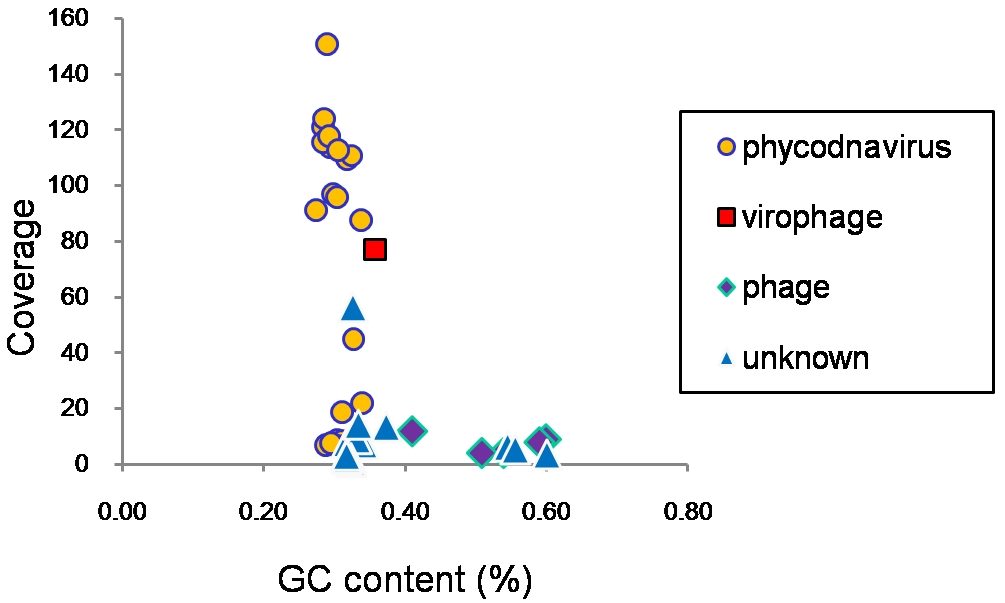
\includegraphics[width=100mm]{olv_figures/olv_GC_plot.jpg}
\caption[Plot of percent GC content \emph{vs} coverage for Organic Lake scaffolds]{ Plot of percent GC content \emph{vs} coverage for the 2006 Organic Lake 0.1 \textmu{}m hybrid assembly scaffolds $>$10 kb.
}
\label{fig:olv_GC_plot}

\end{figure}
 
A broad division was evident between low ($\le$41\%) and high ($\ge$51\%) GC scaffolds suggesting they constituted two taxonomic groups. 
All scaffolds in the high GC group that could be assigned contained phage homologues, as did the one exceptional low GC scaffold. 
The low coverage in the high GC group showed bacteriophages were not abundant in the 0.1 \textmu{}m fraction. 
These scaffolds were not analysed further. 
The low GC scaffolds with confident assignments contained sequences matching conserved \ac{PV} or \ac{ApMV} proteins. 
These \ac{PV}-related scaffolds comprised 60\% of assembled reads demonstrating that \acp{OLPV} were numerically dominant in the 0.1 \textmu{}m fraction. 
\ac{TEM} revealed the presence of virus-like particles with the dimensions and structure typical of PVs (\figreft{fig:TEM}A).
\begin{figure}
\centering
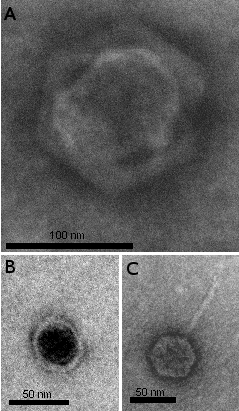
\includegraphics[width=50mm]{olv_figures/TEM.jpg}
\caption[Transmission electron micrographs of Organic Lake \acs{VLP}s]{Transmission electron micrographs of negatively stained \acs{VLP}s from Organic Lake. 
(\textbf{A}) \acs{VLP} resembling the size and morphology of \acs{PV}s,
(\textbf{B}) Sputnik virophage and (\textbf{C}) bacteriophages.
}
\label{fig:TEM}

\end{figure}



Within the low GC group, scaffolds separated into a high coverage ($>$45$\times$) group, including the five longest scaffolds, and a low coverage ($<$22$\times$) group. 
Two of the scaffolds in the high coverage group and one in the low coverage group contained the \ac{PV} marker \ac{DPOB}. 
The two high coverage \ac{DPOB} share 76\% amino acid identity and both share $\sim$57\% identity to the low coverage \ac{DPOB}. 
\ac{DPOB} is single-copy throughout the \ac{NCLDV} family to which \acp{PV} belong \cite{Iyer2001, Iyer2006}, 
demonstrating that the Organic Lake surface waters contained two closely related abundant \ac{PV} types (\ac{DPOB}1) and (\ac{DPOB}2), and a more distantly related lower abundance type (\ac{DPOB}3). 

Phylogenetic analysis clustered Organic Lake \ac{DPOB} with unclassified lytic marine \ac{PV} isolates that infect the prymnesiophytes \emph{Chrysochromulina ericina} (CeV1) and \emph{Phaeocystis pouchetii} (PpV), the prasinophyte \emph{Pyramimonas orientalis} (PoV) \cite{Jacobsen1996, Sandaa2001}, and uncultured marine \acp{PV} related to \ac{ApMV} \cite{Monier2008a, Monier2008b} \figref{fig:OLPV_full_dpo}. 
\begin{figure}
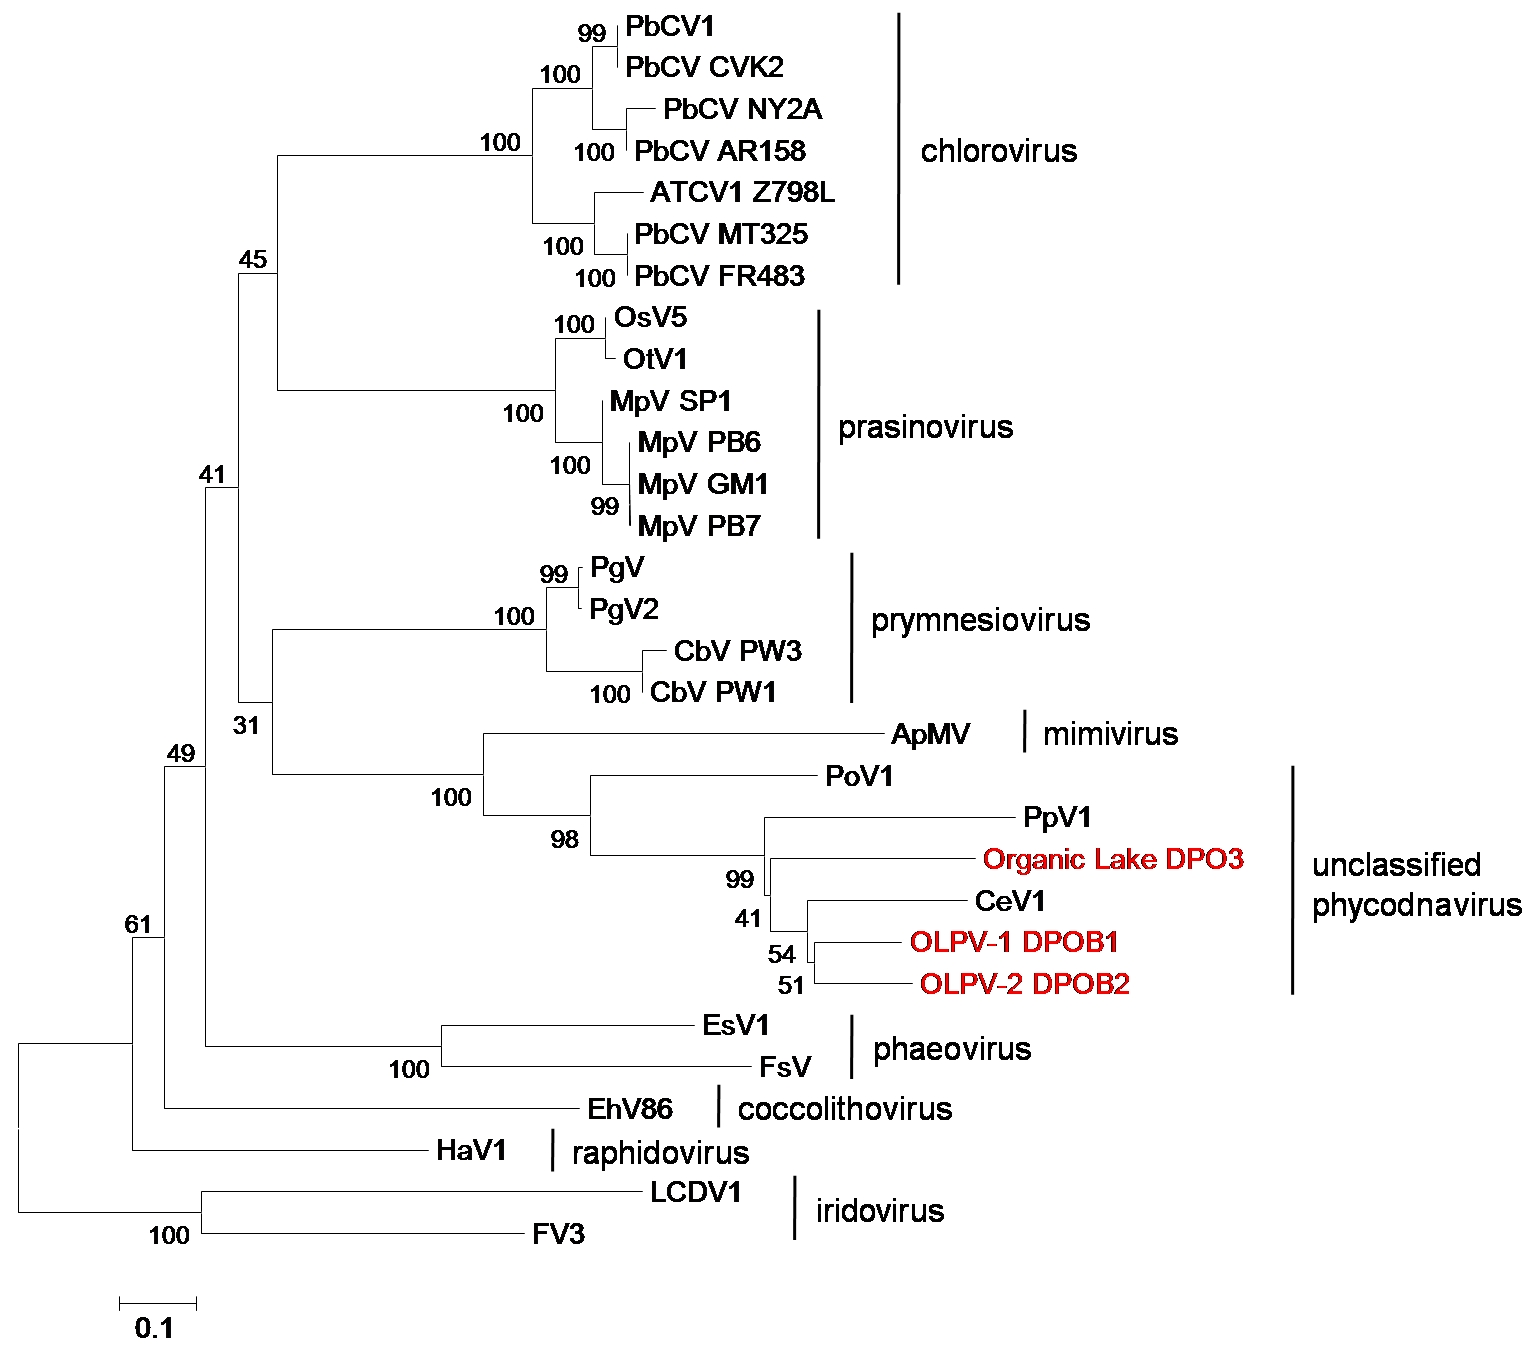
\includegraphics[width=\textwidth]{olv_figures/OLPV_full_dpo.jpg}
\caption[Phylogeny of \ac{OLPV} B family DNA polymerase sequences]{Neighbour-joining tree of B family DNA polymerase amino acid sequences from \ac{OLPV} and \ac{NCLDV} sequences from GenBank. 
Organic Lake sequences are shown in red.
Abbreviations and accession numbers from bottom to top: PbCV1, \emph{Paramecium bursaria} chlorella virus 1 (AAC00532.1); PbCV CVK2, \emph{P. bursaria} chlorella virus CVK2 (BAA35142.1); PbCV NY2A,  \emph{P. bursaria} chlorella virus NY2A (ABT14648.1); PbCV AR158, \emph{P. bursaria} chlorella virus AR158 (ABU43776.1); AtCV1, \emph{Acathocystis turfacea} chlorella virus (ABT16932.1); PbCV MT325,  \emph{P. bursaria} chlorella virus MT325(ABT13573.1); PbCV FR483, \emph{P. bursaria} chlorella virus FR483 (ABT15308.1); OsV5, \emph{Ostreococcus} virus 5 (ABY28020.1); OtV1, \emph{O. tauri} virus 1(YP\_003495047.1);  MpV SP1, \emph{Micromonas pusilla} virus SP1(AAB66713.1); MpV PB6, \emph{M. pusilla} virus PB6 (AAB49743.1); MpV GM1, \emph{M. pusilla} virus GM1 (AAB49742.1); MpV PB7, \emph{M. pusilla} virus PB7 (AAB49744.1); CbV PW1, \emph{Chrysochromulina brevifilum} virus PW1 (AAB49739.1); CbV PW3, \emph{C. brevifilum} virus PW3 (AAB49740.1); ApMV, \emph{Acathamoeba polyphaga} mimivirus (AAV50591.1); PoV,  \emph{Pyramimonas orientalis} virus (ABU23717.1); PpV, \emph{Phaeocystis pouchetii} virus (ABU23718.1); CeV1, \emph{C. ericinia} virus 1 (ABU23716.1); EsV1, \emph{Ectocarpus silicolosus} virus (AAK14511.1); FsV, \emph{Feldmannia} sp. virus (AAB67116.1); EhV86, \emph{Emiliania huxleyii} virus 86 (CAI65453.1); HaV1, \emph{Heterosigma akashiwo} virus 1 (BAE06251.1); FV3, Frog virus 3(AAT09720.1) and LCDV1, Lymphocystis disease virus 1(NP\_078724.1). 
}
\label{fig:OLPV_full_dpo}

\end{figure}

As the host range of \acp{PV} broadly correlates with \ac{DPOB} phylogeny \cite{Nagasaki2005b, Larsen2008}, \acp{OLPV} would infect prasinophytes or prymnesiophytes. 
The most probable host is the prasinophyte, \emph{Pyramimonas} as no prymnesiophyte 18S \ac{rRNA} gene sequences were present in any size fraction of the Organic Lake metagenome \figref{fig:18s}.
\begin{landscape}
\begin{centering}
\begin{figure}
\includegraphics[height=\textheight]{olv_figures/18s.pdf}
\caption[Phylogeny of the 18S rRNA genes from Organic Lake]{Phylogeny of the 18S rRNA genes from the 2006 Organic Lake metagenome. 
Organic Lake sequences are shown in red.
Ace Lake sequences are shown in blue.
}
\label{fig:18s}

\end{figure}
\end{centering}
\end{landscape}


Supporting the presence of more than one \ac{PV}, pairs of single-copy \ac{PV} orthologues 
(ribonucleotide reductase \textalpha{} and \textbeta{} subunits, VV A32R virion packaging helicase, \textsc{PBCV1} A482R-like putative transcription factor, VV D5 ATPase and VLTF2 family transcription factor) 
were identified in the high coverage scaffolds that shared an average of 81\% percent amino acid identity.
 Based on the positions of single copy genes on the scaffolds and the percent identity between them, the high coverage scaffolds were grouped into two strains designated \ac{OLPV}-1 and \ac{OLPV}-2 according to their \ac{DPOB} phylogeny \figref{fig:OLPV_full_dpo}.
 The remaining high coverage scaffolds were assigned to either strain, resulting in two near-complete genomes of $\sim$300 kbp each \figref{fig:OLPV_genome}, that are within the range of other sequenced \ac{PV} genomes (155--407 kbp). 
In addition, several \ac{OLPV} genomic fragments contained \ac{PV} homologues in high coverage scaffolds that could not be confidently assigned to either strain. 
\begin{figure}
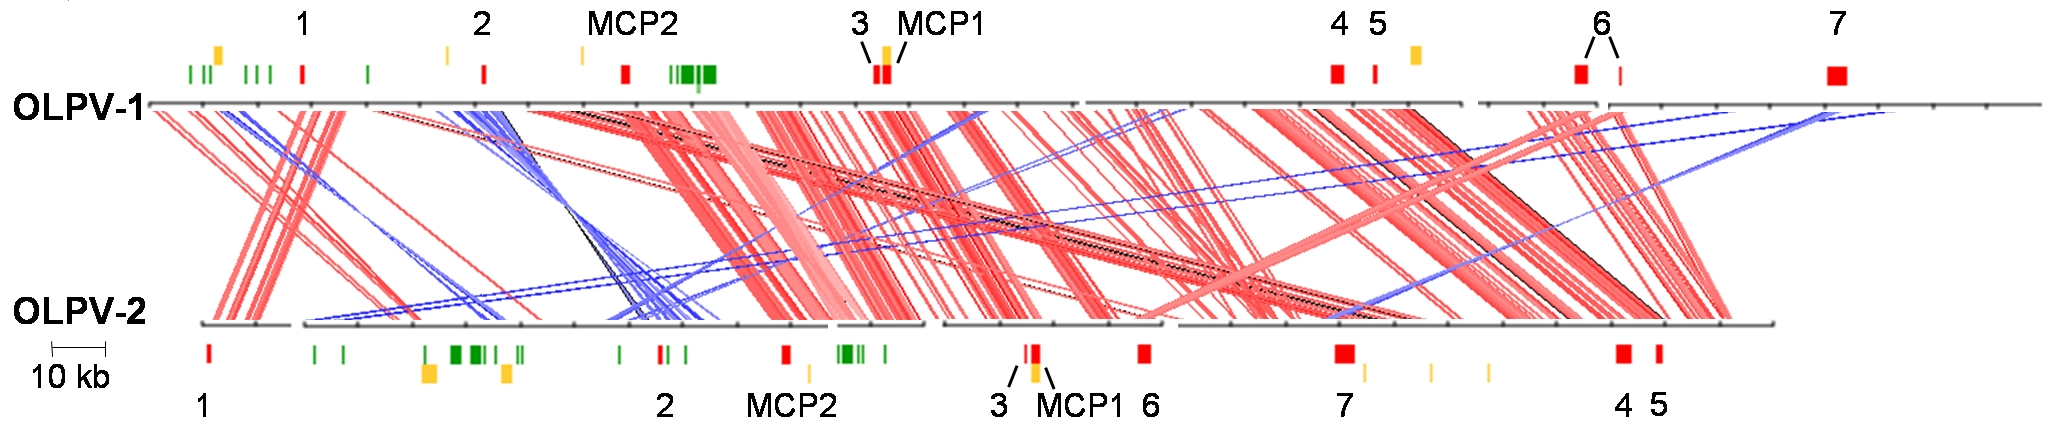
\includegraphics[width=\textwidth]{olv_figures/OLPV_genome.jpg}
\caption[Maps of \acs{OLPV} genomic scaffolds]{Maps of \acs{OLPV}-1 and \acs{OLPV}-2 scaffolds and comparison of the location of genes. Genes are marked as follows: single-copy conserved orthologues and \acs{MCP} (red), regions with identity to \acs{OLV} (green), proteins identified in the metaproteome (yellow), ribosomal nucleotide reductase \textbeta{} (1), VV A32 packaging ATPase (2), VV VLTF3 transcription factor (3), VV D5 replicative helicase (4), PbCV-1 A482R-like putative transcription factor (5), ribonucleotide reductase \textalpha{} (6), and \textsc{DNA} polymerase B (7). Lines connect homologous regions between the \ac{OLPV}-1 and \ac{OLPV}-2 scaffolds in the same orientation (red) and reverse orientation (blue).
}
\label{fig:OLPV_genome}

\end{figure}


Both \ac{OLPV} strains contain a PpV-like \ac{MCP} designated \ac{MCP}1 and another unique \ac{MCP} designated \ac{MCP}2 \figref{fig:OLPV_full_mcp}.
\begin{figure}
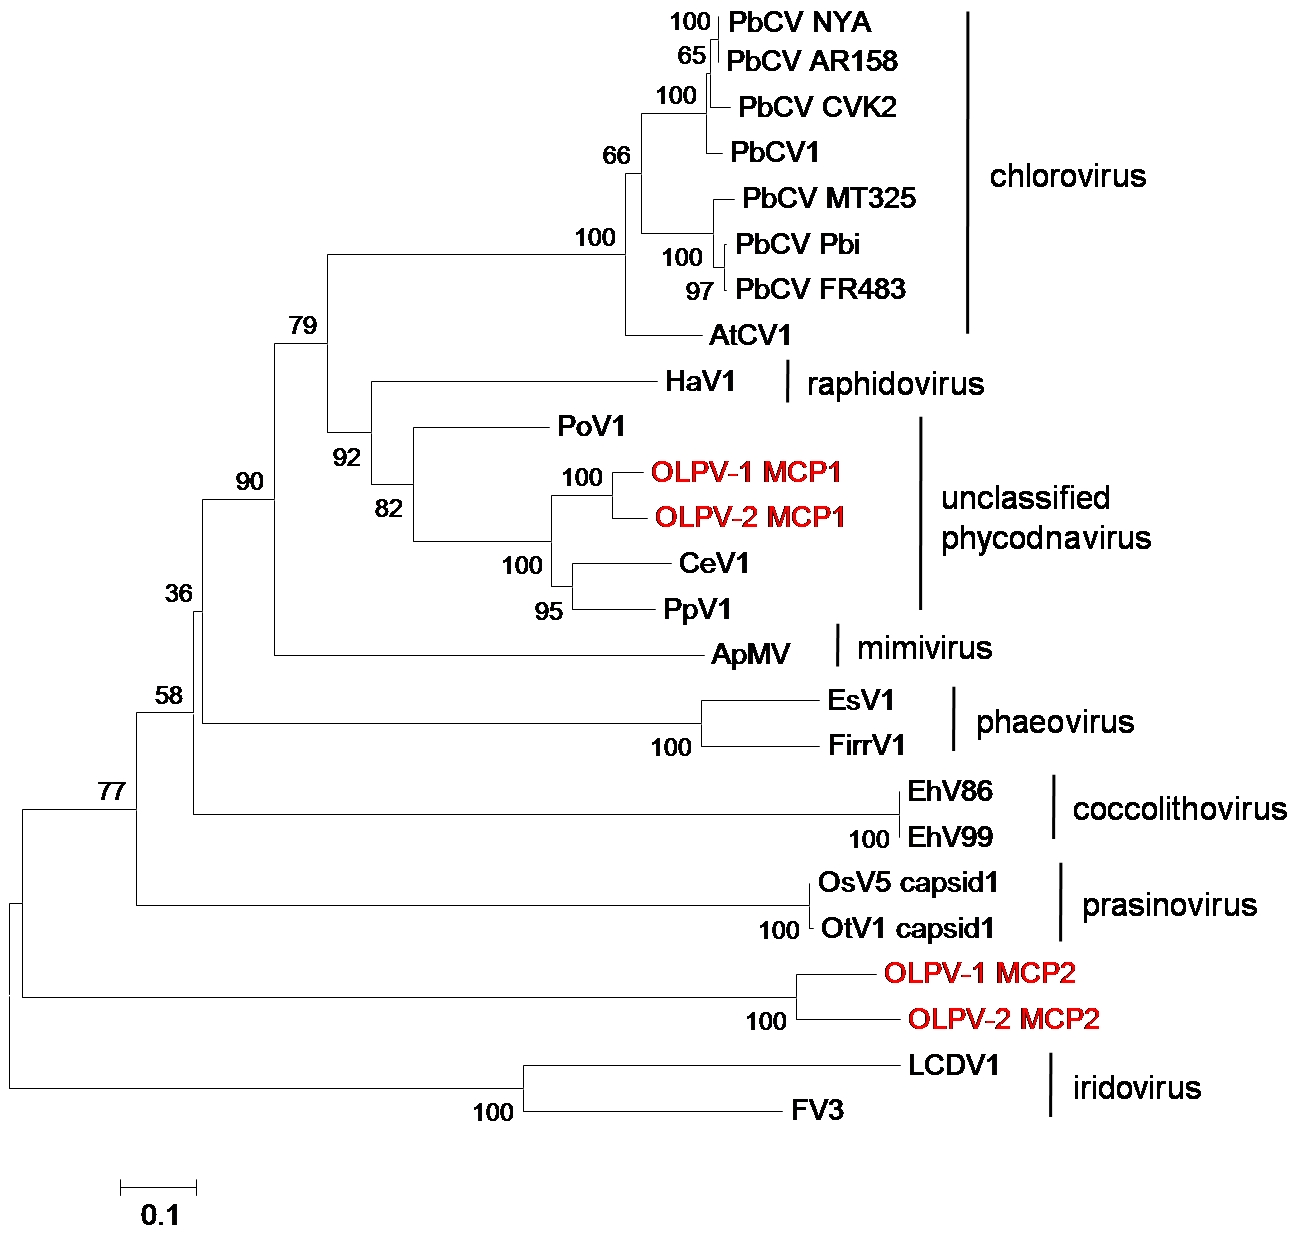
\includegraphics[width=\textwidth]{olv_figures/OLPV_full_mcp.jpg}
\caption[Phylogeny of \acs{OLPV} major capsid protein sequences]{Neighbour-joining tree of major capsid protein amino acid sequences from \ac{OLPV} and  other \acs{NCLDV} sequences from GenBank. 
Abbreviations and accession numbers from top to bottom: PbCV NYA, \emph{Paramecium bursaria} chlorella virus NY2A (ABT14984.1); PbCV AR158, \emph{P. bursaria} chlorella virus AR158 (ABU44077.1); PbCV CVK2, \emph{P. bursaria} chlorella virus CVK2 (BAA35143.1); PbCV1, \emph{P. bursaria} chlorella virus 1(AAA88828.1); PbCV MT325, \emph{P. bursaria} chlorella virus MT325 (ABT14017.1); PbCV Pbi, \emph{P. bursaria} chlorella virus Pbi (AAC27492.1); PbCV FR483, \emph{P. bursaria} chlorella virus FR483 (ABT15755.1); AtCV1, \emph{Acathocystis turfacea} chlorella virus 1 (ABT16414.1); HaV1, \emph{Heterosigma akashiwo} virus 1 (BAE06835.1); PoV, \emph{Pyramimonas orientalis} virus (ABU23714.1); CeV1, \emph{Chrysochromulina ericinia} virus 1 (ABU23712.1); PpV1, \emph{Phaeocystis pouchetii} virus (ABU23715.1); ApMV, \emph{Acathamoeba polyphaga} virus (Q5UQL7.2); EsV1, \emph{Ectocarpus siliculosus} virus (AAK14534.1); FirrV1, \emph{Feldmannia irregularis} virus 1 (AAR26925.1); EhV86, \emph{Emiliania huxleyi} virus 86 (CAI65508.2); EhV99, \emph{E. huxleyi} virus 99 (ABU23713.1); OsV5, \emph{Ostreococcus} virus 5 (ABY27849.1); OtV1, \emph{O. tauri} virus 1 (CAY39653.1); LCDV1, Lymphocystis diseases virus 1(AAC24486.2); FV3, Frog virus 3 (AAT09750.1). 
}
\label{fig:OLPV_full_mcp}

\end{figure}

Both \ac{OLPV} \ac{MCP}1s were identified in the metaproteome (\figreft{fig:OLPV_genome} and \tabreft{tab:pmics}) but \ac{MCP}2 was not. 
In addition to \acp{MCP}, the metaproteome contained a range of abundant structural proteins and others more likely to be packaged in the virion (e.g. chaperone), that were expressed by \ac{OLPV}-1, \ac{OLPV}-2 and/or an \ac{OLPV} genomic fragment \tabreft{tab:pmics}. 
These data suggest that \ac{MCP}1 is the major structural protein, and that both \ac{OLPV}-1 and \ac{OLPV}-2 were in a productive cycle in the lake at the time of sampling. 
\begingroup
\begin{table}
\footnotesize
\caption[OLPV and OLV proteins identified in the metaproteome]{OLPV and OLV proteins identified in the December 2006 0.1 \textmu{}m size fraction metaproteome. Peptide sequences by which the proteins were identified are shown in Appendix \tabreft{tab:peptides}. NSA, normalised spectral abundance; Cov., coverage. $a$Proteins that have some shared peptides; $b$162322406 and 162276024 are protein homologues; $c$A group of proteins containing similar peptides that could not be differentiated by the mass spectral analysis. Only one gene number of that groups is displayed.}
\label{tab:pmics}
\smallskip
\begin{tabularx}{\textwidth}{p{1.3cm}p{1.2cm}p{1cm}p{1.8cm}p{4.7cm}p{0.4cm}p{1.4cm}}
\toprule
\textbf{Gene ID} & \textbf{Source} & \textbf{NSA} & \textbf{Accession} & \textbf{Description} & \textbf{Cov. (\%)} & \textbf{Peptides (unique)} \\
\midrule
162322530$a$ & OLPV-1 & 0.000661 & A7U6F0 & Major capsid protein & 33 & 15 (4) \\
 &  &  &  & [\emph{Phaeocystis pouchetii} virus] &  & \\
162322348 & OLPV-1 & 0.000120 & - & - & 11.3 & 2 (2) \\
162322406$b$ & OLPV-1 & 0.000177 & - & - & 29.4 & 4 (4) \\
162313481 & OLPV-1 & 0.000010 & YP\_002714448 & Leucine rich repeat-containing & 3.96 & 2 (2) \\
 &  &  &  & Miro-like protein & & \\
 &  &  &  & [\emph{Synechococcus} sp. PCC7335] &  & \\
162276060 & OLPV-2 & 0.000897 & - & - & 28.9 & 2 (2) \\
162300260 & OLPV-2 & 0.000226 & - & - & 34.6 & 2 (2) \\
162276024$b$ & OLPV-2 & 0.000127 & - & - & 16 & 3 (3) \\
162275992 & OLPV-2 & 0.000098 & NP\_048709 & Hypothetical protein & 16.6 & 2 (2) \\
 &  &  &  & PBCV1\_A352L [\emph{Paramecium} & &  \\
 &  &  &  & \emph{bursaria} chlorella virus 1] & &  \\
162300108 & OLPV-2 & 0.000046 & ZP\_01471812 & BNR containing hypothetical protein RS9916\_28494 & 7.66 & 5 (5) \\
 &  &  &  & [\emph{Synechococcus} sp. RS9916] &  &  \\
162319393$a$ & OLPV-2 & 0.000016 & A7U6F0 & Major capsid protein & 26.3 & 13 (2) \\
 &  &  &  & [\emph{Phaeocystis pouchetii} virus] &  &  \\
162300134$c$ & OLPV- & 0.00010 & AAR21578 & Heat shock protein 70 & 6.97 & 3 (3) \\
 & 1/2  &  &  & [\emph{Phytophthora nicotianae}] &  &  \\
162286324$c$ & OLPV & 0.000176 & NP\_048575 & Hypothetical protein & 14.7 & 2 (2) \\
 &  &  &  & PBCV1\_A227L [\emph{Paramecium} &  &  \\
 &  &  &  & \emph{bursaria} chlorella virus 1] &  &  \\
OLV9 & OLV & 0.001681 & YP\_002122381 & Capsid protein V20 & 31.1 & 15 (15) \\
 &  &  &  & [Sputnik virophage] &  &  \\
OLV8 & OLV & 0.000334 & YP\_002122379 & N-term: hypothetical protein V18 [Sputnik virophage]   & 19.1 & 8 (8) \\
 &  &  & YP\_002122380 &  C-term: minor capsid protein V19 [Sputnik virophage]  &  &  \\
\bottomrule
\end{tabularx}
\end{table}
\endgroup



\subsection{Complete genome of an Organic Lake virophage}
Sputnik is a small (50 nm) icosahedral satellite virus of mamavirus (a new strain of \ac{ApMV}). 
It was termed a virophage because co-infection with Sputnik is deleterious to the mamavirus, resulting in abnormal virions and a decrease in mamavirus infectivity \cite{LaScola2008}. 
One 28 kbp scaffold in the low GC high coverage group had six out of 38 predicted proteins homologous to Sputnik virophage proteins (\figreft{fig:OLV_genome} and \tabreft{tab:olv_annotation}), and one \ac{PV} homologue. 
The scaffold had a low GC content ($\sim$30\%), similar to the Sputnik genome, and was larger in size (28 kbp vs 18 kbp for Sputnik). 
Using \ac{PCR} and sequencing, the scaffold was found to represent a complete circular virophage genome.
This shows the Organic Lake genome has the same circular topology as the Sputnik genome \cite{LaScola2008}. 
Virus-like particles resembling Sputnik in size and morphology were identified by \ac{TEM} (\figreft{fig:TEM}B).
\begin{figure}
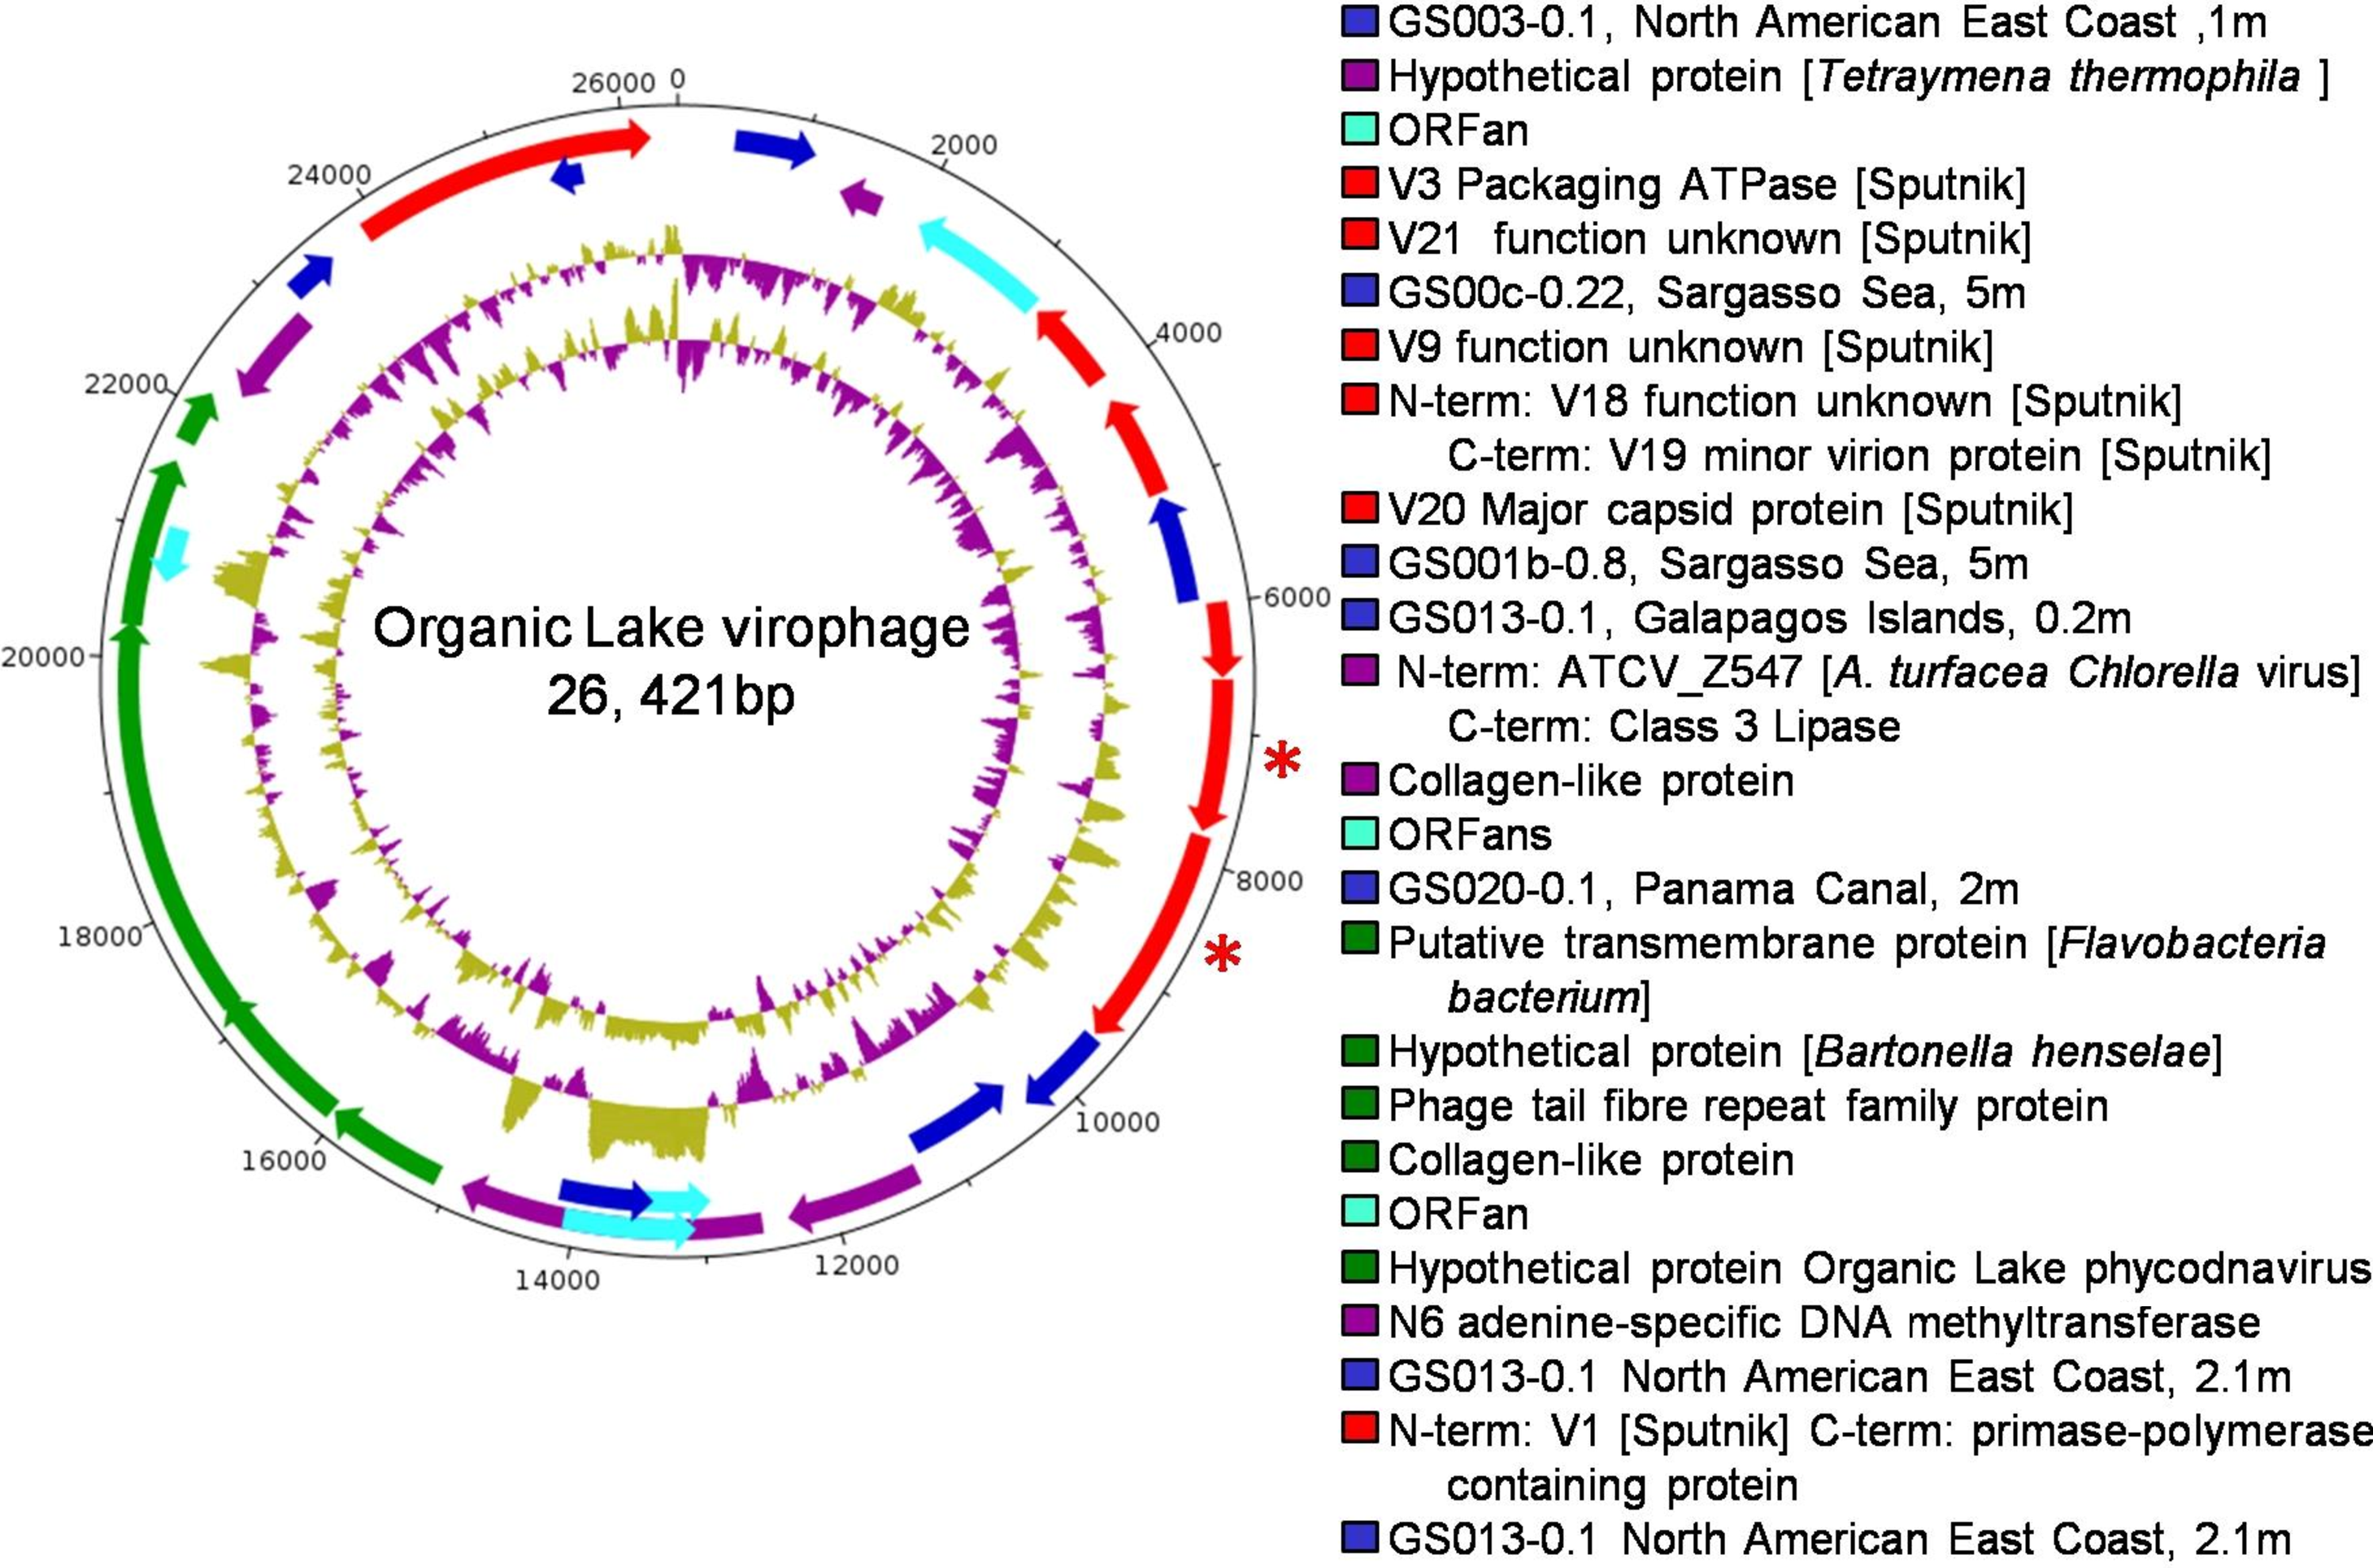
\includegraphics[width=\textwidth]{olv_figures/OLV_genome.pdf}
\caption[Genomic map of Organic Lake virophage]{Genomic map of Organic Lake virophage. From the outside-in, circles represent, 1) predicted coding sequences on the forward strand, 2) predicted coding sequences on the reverse strand, 3) GC skew, and 4) GC plot. Predicted coding sequences are coloured: Sputnik homologues (red), OLPV homologues (green), non-Sputnik \ac{NR} homologues (purple), \ac{GOS} peptide database homologues (blue), and ORFan (cyan). Sequences identified in the metaproteome are marked with an asterisk. Descriptions of the predicted coding sequences from both strands are shown clockwise from position zero.
}
\label{fig:OLV_genome}

\end{figure}

\begin{landscape}
\begingroup
\footnotesize
\begin{longtable}{p{0.7cm}p{0.7cm}p{0.7cm}p{8cm}p{5cm}p{7cm}}
\caption[Annotation of Organic Lake virophage genome ]{Annotation of Organic Lake virophage genome. Top \textsc{BLASTp} matches of predicted coding sequences from the \ac{OLV} genome compared to \ac{OLPV}, \ac{NR} protein database, and \ac{CAMERA} metagenomic reads \ac{ORF} peptide database.}
\label{tab:olv_annotation}
\\
\toprule
\textbf{Gene ID} & \textbf{Start} & \textbf{End} &\textbf{NR (acc, \%ID, e-value)} & \textbf{OLPV (geneID, \%ID, e-value)} & \textbf{CAMERA (acc, \%ID, e-value)} \\
\midrule
\endfirsthead
\multicolumn{6}{c}
{\tablename\ \thetable\ -- \textit{Continued from previous page}} \\
\toprule
\textbf{Gene ID} & \textbf{Start} & \textbf{End} &\textbf{NR (acc, \%ID, e-value)} & \textbf{OLPV (geneID, \%ID, e-value)} & \textbf{CAMERA (acc, \%ID, e-value)} \\
\midrule
\endhead
\bottomrule \multicolumn{6}{r} {\textit{Continued on next page}} \\
\endfoot
\bottomrule
\endlastfoot
OLV1 & 460 & 1,077 & - & - & GS003, 0.1, North America East Coast, 1 m\\
 &  &  &  &  & (JCVI\_PEP\_1105157870626/41\%/1e$-$29)\\

OLV2 & 1,701 & 1,333 & Hypothetical protein [\emph{Tetrahymena thermophila} SB210]  & - & GS012, 0.1, North American East Coast, 13.2 m \\
 &  &  & (XP\_001029204.1/38\% /3e$-$04) &  & (JCVI\_PEP\_1105080106223/42\%/1.7e$-$11)\\

OLV3 & 3,187 & 2,030 & - & - & -\\

OLV4 & 3,991 & 3,224 & - & - & -\\

OLV5 & 5,029 & 4,160 & V3 [Sputnik virophage] & - & GS001b, 0.8, Sargasso Sea, 5 m \\
 &  &  & (YP\_002122364.1/ 39\%/4e$-$24) &  & (JCVI\_PEP\_1105131296011/43\%/5e$-$38) \\

OLV6 & 5,940 & 5,044 & - & - & GS000c, 0.22, Sargasso Sea, 5m \\
 &  &  &  &  & (JCVI\_PEP\_1105136847382/24\%/6e$-$3) \\

OLV7 & 5,978 & 6,547 & V9 [Sputnik virophage] & - & GS020, 0.1, Panama Canal, 2 m \\
 &  &  & (YP\_002122370.1/35\%/3e$-$14) &  & (JCVI\_PEP\_1105140820785/26\%/1e$-$12) \\

OLV8 & 6,574 & 7,740 & N-term: V18 [Sputnik virophage]  & - &  GS008, 0.1, North American East Coast, 1 m \\
 &  &  &  (YP\_002122379.1/27\%/9e-05)  &  & (JCVI\_PEP\_1105124194533/32\%/6e$-$8) \\
 &  &  & C-term: V19 [Sputnik virophage] &  & - \\
 &  &  & (YP\_002122380.1/26\%/0.16) &  &  \\

OLV9 & 7,791 & 9,518 & V20 [Sputnik virophage] & - & GS033, 0.1, Galapagos Islands, 0.2 m \\
 &  &  & (YP\_002122381.1/28\%/9e-10) &  & (JCVI\_PEP\_1105120114513/28\%/2e$-$14) \\

OLV10 & 9,563 & 10,273 & - & - & GS001b, 0.8, Sargasso Sea, 5 m \\
 &  &  &  &  & (JCVI\_PEP\_1105163928413/61\%/5e$-$4) \\

OLV11 & 11,210 & 10,317 & - & - & GS013, 0.1, North America East Coast, 2.1 m \\
 &  &  &  &  & (JCVI\_PEP\_1105123792445/39\%/9e$-$37) \\

OLV12 & 11,284 & 12,324 & N-term: Hypothetical protein ATCV\_Z547R  & - & GS018, Carribean Sea, 1.7 m \\
 &  &  & [\emph{Acanthocystis turfacea} chlorella virus 1]  &  &  (JCVI\_PEP\_1105087988121/34\%/5.6e$-$23) \\
 &  &  & (YP\_001427028.1/36\%/7e$-$09)  &  &  \\
 &  &  & C-term: Lipase class 3 [\emph{Bacillus thuringiensis} IBL200]  & - & - \\
 &  &  & (EEM96541.1/27\%/1.7e$-$02)  &  &  \\


OLV13 & 12,539 & 14,884 & Collagen-like protein [\emph{Bacillus megaterium}] & - & GS027, 0.1, Galapagos Islands, 2.2m \\
 &  &  &  (YP\_001569009.1/66.67\%/4e$-$03) &  & (JCVI\_PEP\_1105075498120/43\%/6.7e$-$11) \\

OLV14 & 14,023 & 12,905 & - & - & - \\
OLV15 & 13,041 & 14,078 & - & - & - \\
OLV16 & 15,094 & 13,372 & - & - & GS020, 0.1, Panama Canal, 2 m \\
 &  &  &  &  & (JCVI\_PEP\_1105127133835/36\%/8.5e$-$11) \\

OLV17 & 15,094 & 16,023 & Putative transmembrane protein  & Lipoprotein Q-like protein  & GS009, 0.1, North American East Coast, 1 m \\
 &  &  & [\emph{Flavobacteria} bacterium BAL38] &  (162322444/40\%/1e$-$24) & (JCVI\_PEP\_1105137954859/50\%/4e$-$37) \\
&  &  & (ZP\_01734433.1/51\%/8e$-$34) &  &  \\

OLV18 & 16,054 & 17,211 & Hypothetical protein BH13620 & \emph{Cyanothece} sp. cce\_0037-like & GS000c, 0.1, Carribean Sea, 2 m \\
 &  &  & [\emph{Bartonella henselae} str. Houston-1]  &  protein (162322244/65\%/2e$-$33) & (JCVI\_PEP\_1105149563549/39\%/2e$-$26) \\
 &  &  &  (YP\_034083.1/15\%/4e$-$04) &  &  \\

OLV19 & 17,168 & 20,278 & Phage tail fiber repeat family protein & Lipoprotein Q-like protein & GS016, 0.1, Carribean Sea, 2 m \\
 &  &  & [\emph{Trichomonas vaginalis} G3] & (162322444/65\%/9e$-$33) & (JCVI\_PEP\_1105149563549/29\%/1e$-$27)\\
 &  &  & (XP\_001296018.1/42\%/4e$-$11) &  & \\

OLV20 & 20,266 & 21,570 & Collagen triple helix containing protein A1Q\_3499 & Hypothetical protein & GS033, 0.1, Galapagos Islands, 0.2 m \\
 &  &  & [\emph{Vibrio harveyi} HY01] & (162322252/32\%/1e$-$07) & (JCVI\_PEP\_1105153074955/69\%/1e$-$5) \\
 &  &  & (ZP\_01986098.1/69\%/6e$-$04) &  &  \\

OLV21 & 21,089 & 20,622 & - & - & - \\
OLV22 & 21,747 & 22,157 & - & Hypothetical protein & GS017, 0.1, Carribean Sea, 2 m \\
 &  &  &  & (162322266/56\%/5e$-$31) & (JCVI\_PEP\_1105100448171/43\%/4e$-$24) \\

OLV23 & 23,089 & 22,256 & D12 class N6 adenine-specific DNA methyltransferase & - & GS002, 0.1, North America East Coast, 1 m \\
 &  &  &  [``\emph{Candidatus} Koribacter versatlis'' Ellin345] &  & (JCVI\_PEP\_1105085453201/33\%/8e$-$18) \\
 &  &  & (YP\_592471.1/28\%/1e$-$24) &  &  \\

OLV24 & 23,174 & 23,560 & - & - & GS013, 0.1,  North American East Coast 2.1 m \\
 &  &  &  &  & (JCVI\_PEP\_1105132174179/32\%/1e$-$03) \\

OLV25 & 23,889 & 26,219 & N-term: V13 [Sputnik virophage] & - & GS030, 0.1, Galapagos Islands, 19 m   \\
 &  &  & (YP\_002122374.1/34\%/5e$-$31) &  & (JCVI\_PEP\_1105105378071/40\%/8e$-$38)  \\
 &  &  & C-term: Primase-polymerase domain containing hypothetical protein  &  & GS013, 0.1, North America East Coast, 2.1 m  \\
 &  &  & [\emph{Ostreococcus lucimarinus} CCE9901]  &  & (JCVI\_PEP\_1105129419397/51\%/8e$-$71) \\
 &  &  & (XP\_001421479.1/29\%/9e$-$32) &  &  \\

OLV26 & 25,666 & 25,376 & - & - & GS013, 0.1, North American East Coast, 2.1 m  \\
 &  &  &  &  & (JCVI\_PEP\_1105129419399/54\%/8e$-$6) \\

\end{longtable}
\endgroup
\end{landscape}


Sputnik homologues present in the Organic Lake scaffold included the V20 \ac{MCP}, V3 \textsc{DNA} packaging \textsc{ATP}ase, V13 putative \textsc{DNA} polymerase/primase and others of unknown function (V9, V18, V21 and V32) (\figreft{fig:OLV_genome} and \tabref{tab:pmics}). 
The \ac{OLV} is distinct to Sputnik as proteins share 27--42\% amino acid identity (28\% \ac{MCP} identity). 
\ac{OLV} proteins include OLV9, the homologue of Sputnik V20 \ac{MCP}, and OLV8, a fusion of the uncharacterised V18 and minor virion protein V19 from Sputnik (\figreft{fig:OLV_genome} and \tabreft{tab:olv_annotation}). 
The large number of homologues, including genes that fulfill essential functions in Sputnik (V20, V3 and V13), indicate that \ac{OLV} and Sputnik have physiological similarities. 

\subsection{Gene exchange between virophage and phycodnaviruses}

As \acp{PV} are related to \ac{ApMV} \cite{Iyer2006} and are abundant in Organic Lake, it stands to reason that \ac{OLPV} is the helper of \ac{OLV}. 
In the \ac{OLV} genome, OLV12 is a chlorella virus-derived gene, indicating that gene exchange has occurred between \ac{OLV} and \acp{PV} (the function of OLV12 is discussed below).
Similar observations were made for Sputnik, which carries four genes (V6, V7, V12 and V13) in common with the mamavirus, indicative of gene exchange between the viruses and possible co-evolution \cite{LaScola2008}. 
As the V6, V7, V12 and V13 proteins have been associated with virophage--helper specificity, we reasoned that the functional analogues in \ac{OLV} would have highest identity to proteins from its helper virus, rather than Sputnik. 

By comparing \ac{OLV} and \ac{OLPV}, a 7,408 bp region was identified in \ac{OLV} encoding five proteins (OLV17--22) with identity (32--65\%) to sequences in both \ac{OLPV}-1 and \ac{OLPV}-2 (\figreft{fig:OLPV_genome}, \figreft{fig:OLV_OLPV_compare} and \tabreft{tab:olv_annotation}). 
\begin{figure}
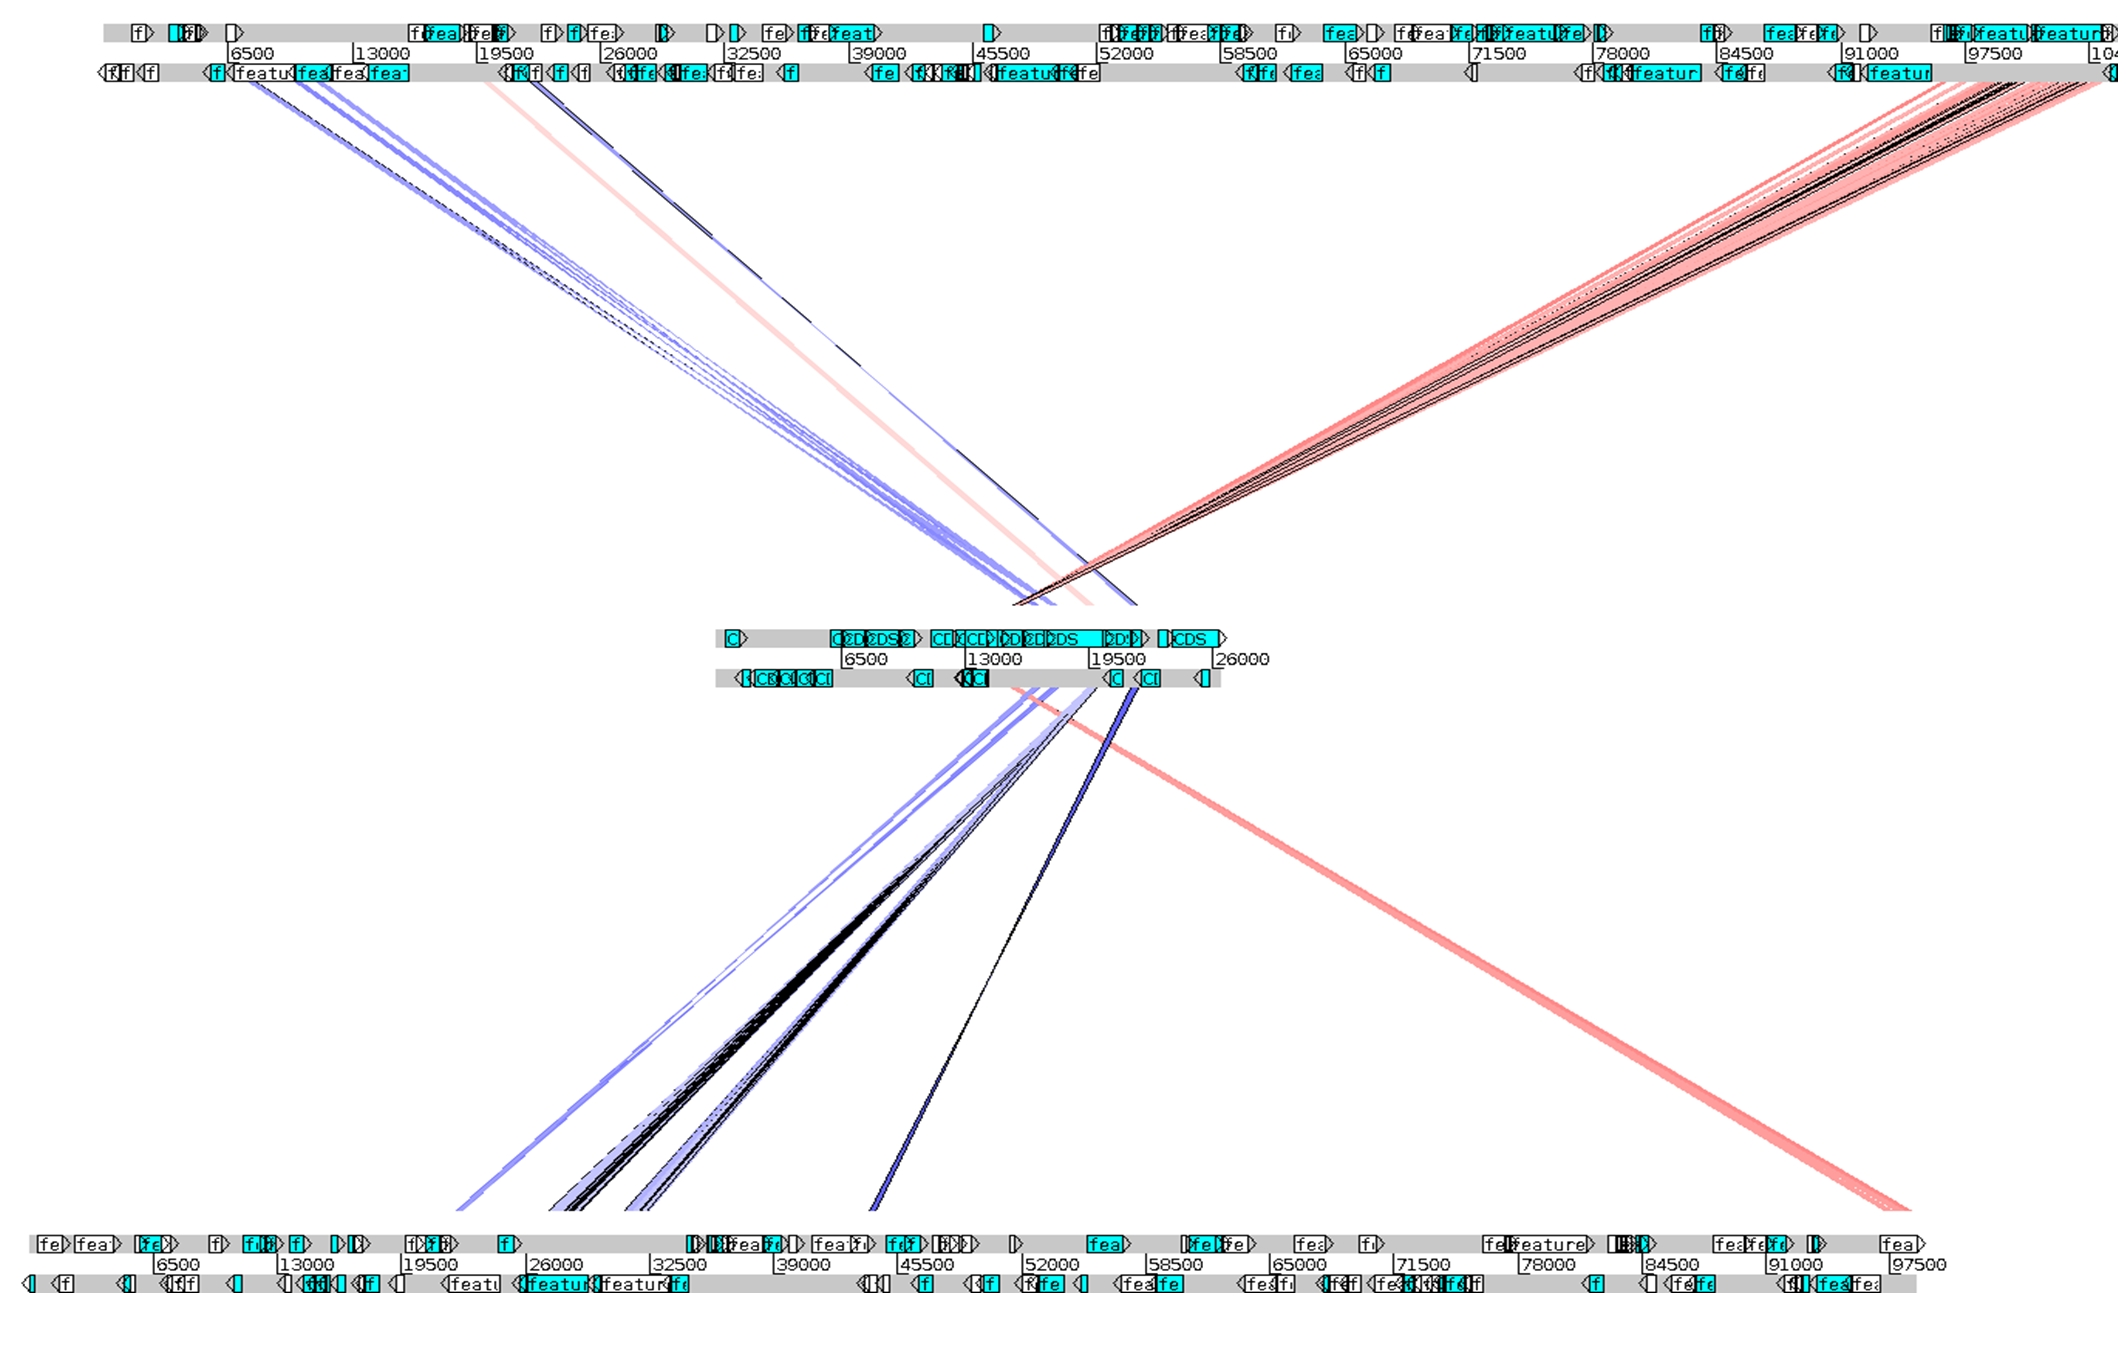
\includegraphics[width=\textwidth]{olv_figures/OLV_OLPV_compare.jpg}
\caption[Genomic comparison of \acs{OLV} and \acs{OLPV}s]{Comparison of the location of genes in \ac{OLV} compared to \acs{OLPV}s. \ac{OLV} (centre), \acs{OLPV}-1 (top), and \acs{OLPV}-2 (bottom).
}
\label{fig:OLV_OLPV_compare}

\end{figure}

OLV20 and OLV13 are collagen triple-helix-repeat-containing proteins, analogous to Sputnik collagen-like proteins (V6 and V7) involved in protein--protein interactions in the \ac{ApMV} virus factory. 
Sputnik can replicate with either mamavirus or \ac{ApMV} as a helper, although coinfection rates are higher with the mamavirus. 
V6 is the only protein with higher identity (69\%) to mamavirus than \ac{ApMV} (42\%) \cite{LaScola2008}. 
Since OLV20 has equivalent identity (63\%) with \ac{OLPV}-1 and \ac{OLPV}-2, it appears that \ac{OLV} may be capable of interacting with both \ac{OLPV} strains. 
Also within the conserved region, OLV22, is a 141 aa protein of unknown function that only matches sequences from \ac{OLPV} and the \ac{GOS} expedition \tabref{tab:olv_annotation}. 
Similar to OLV22, Sputnik V12 is a small protein (152 aa) of unknown function with high identity to \ac{ApMV}, and both may mediate a specific helper--virophage interaction. 
Other genes in this region of \ac{OLV} can be mapped to \ac{OLPV}, including a putative transmembrane protein (OLV17) and paralogous phage tail fibre repeat containing proteins, OLV18 and OLV19. 
Analogous to the collagen-like proteins, OLV19 and OLV20 probably facilitate interactions between helper and virophage. 

OLV12, which is unique to \ac{OLV}, consists of a C-terminal domain present in conserved hypothetical chlorella virus proteins and an N-terminal domain most closely related to class 3 lipases that may confer \ac{OLV} selectivity to a \ac{PV}. 
OLV12 may function similarly to the Sputnik V15 membrane protein in modifying the \ac{ApMV} membrane \cite{LaScola2008}. 
The Sputnik V13 consists of a primase domain and SF3 helicase domain related to \ac{NCLDV} homologues, involved in \textsc{DNA} replication. 
The helicase domain of OLV25 and V13 are similar, although the primase domain is more similar to a protein from \emph{Ostreococcus lucimarinus}, implying a past association of \ac{OLV} with a prasinophyte alga host. 

Genes unique to \ac{OLV} point to adaptations specific to its helper--host system. 
Most notably, \ac{OLV} possesses a N6 adenine-specific \textsc{DNA} methyltransferase, as does \ac{OLPV}. 
In \ac{OLPV}-1, genes for a bacterial type I \ac{RM} system are adjacent to a gene encoding a type I methylase-S target recognition domain protein, and upstream of a \textsc{DNA} helicase distantly related to type III \ac{RE} subunits. 
A large number of chlorella virus genomes have both 5mC and 6mA methylation \cite{VanEtten1991}, and several contain functional \ac{RM} systems \cite{Nelson1993}. 
The prototype chlorella virus PbCV-1 possesses REs packaged in the virion for degrading host \textsc{DNA} soon after infection \cite{Agarkova2006}. 
In contrast to \ac{OLV} and \ac{OLPV}, \textsc{DNA} methyltransferases are absent in both Sputnik and \textsc{ApMV}, indicating that the N6 adenine-specific \textsc{DNA} methyltransferase has been selected in \ac{OLV} to reduce endonucleolytic attack mediated by \ac{OLPV}. 

\subsection[Virophage in algal host--phycodnavirus dynamics]{Role of virophage in algal host--phycodnavirus dynamics}
The presence of the virophage adds an additional consideration to the microbial loop dynamics. 
In batch amoeba cultures, co-infection of amoeba with \ac{ApMV} and Sputnik causes a 70\% decrease in infective \ac{ApMV} particles and a 3-fold decrease in lysis \cite{LaScola2008}. 
To test how \ac{OLV} affects \ac{OLPV} and host population dynamics, we modelled the \ac{OLV} as an additional predator of a predator in a Lotka-Volterra simulation \figref{fig:LV}.
 
The classic Lotka-Volterra model \cite{Lotka1910} is based on a pair of first-order, non-linear, differential equations that can be used to describe the periodic oscillation of the populations of a predator and its prey \cite{Volterra1926}. 
An example of how predator (virus) populations follows that of its prey (host) populations over time is shown in \figreft{fig:LV}A where the populations are at equilibrium.
The extended model shown (\figreft{fig:LV}C) is based on three equations describing the host (prey), virus (predator) and virophage (predator of predator) interactions. 
In this model, the effect of virophage is robust, with equilibrium solutions across a wide range of parameter values (\figreft{fig:LV}C shows one equilibrium solution).
It shows the virus population following that of it host and the virophage population in turn following that of its helper virus or ``host''. While the absolute number of hosts do not increase greatly as a result of \ac{OLV} preying on \ac{OLPV}, the frequency of host blooms increases in the presence of \ac{OLV}. 
\begin{figure}
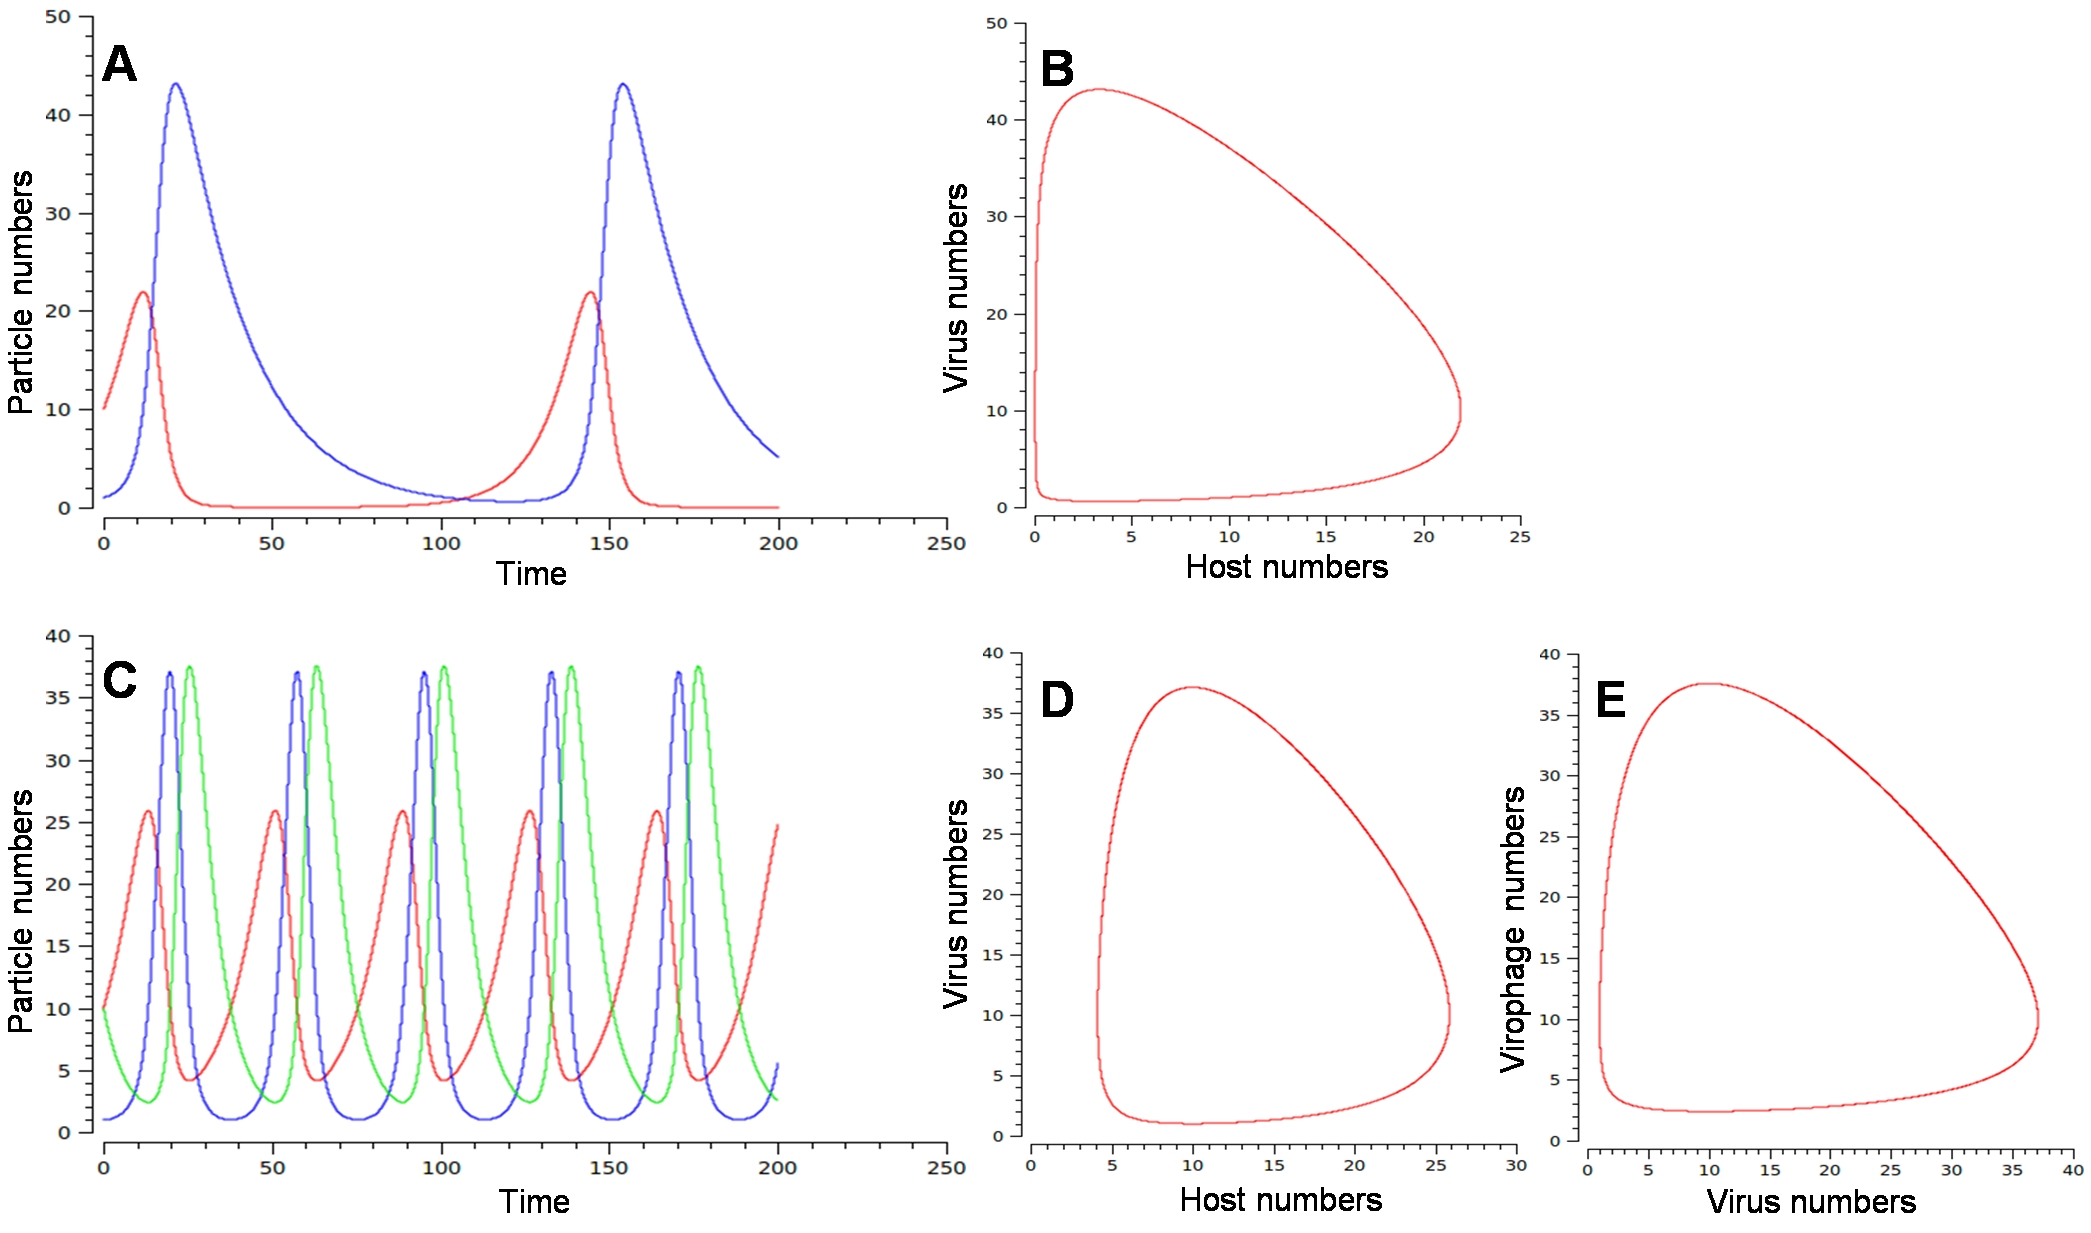
\includegraphics[width=\textwidth]{olv_figures/LV.jpg}
\caption[Extended Lotka-Volterra models of host--OLPV--OLV population dynamics]{Extended Lotka-Volterra models of host--OLPV--OLV population dynamics. 
(\textbf{A}) Time course of host (red line) and \ac{OLPV} (blue line) populations in the absence of \ac{OLV}. 
(\textbf{B}) Orbit plot between host and \ac{OLPV} populations in the absence of \ac{OLV} with the host and \ac{OLPV} populations approaching zero during an equilibrium cycle. 
(\textbf{C}) Time course describing the effect of the addition of \ac{OLV} (green line) on OLPV-host population dynamics as a predator of predator resulting in increased frequency of population ocillations and a higher minimal number of hosts and \acp{OLPV} (\textbf{D}) compared to in the absence of OLV (\textbf{B}). 
(\textbf{E}) The orbit plot of \ac{OLPV} and \ac{OLV} is also shown. 
Note that the time intervals are arbitrary.
}
\label{fig:LV}

\end{figure}


This is due to \ac{OLV} decreasing the number of infective \acp{OLPV}, thereby shortening the recovery time of the host population (\figreft{fig:LV}C).
This is evident in the orbit plot (\figreft{fig:LV}D) as the shift of the orbit away from the axis. 

The model reveals that the virophage stimulates the flux of secondary production through the microbial loop by reducing overall mortality of the host algal cell following a bloom, and by increasing the frequency of blooms during the summer light periods. 
Antarctic lake systems have evolved mechanisms to cope with long light-dark cycles \cite{Lauro2011} and shortened trophic chains. 
In Organic Lake and similar systems, a decrease in \ac{PV} virulence may be instrumental in maintaining stability of the microbial food web. 
In other words, the increased turnover in the microbial loop during the extended light periods of the polar summer may help to maintain microbial populations in the lake.

\subsection{Ecological relevance of virophages in aquatic systems}
Metagenomic analysis of Organic Lake samples taken two years later in November (when the lake was ice covered) and December 2008 (partially ice-free) revealed sequences with 99\% amino acid identity to \ac{OLV} \ac{MCP} indicating persistence of \ac{OLV} in the ecosystem (\figreft{fig:OLV_time} and \tabreft{tab:olv_mcp_blastp}). 
In addition, sequences with lower identity (25--90\%) were detected, particularly in December, demonstrating Organic Lake virophages are highly diverse but \ac{OLV} remained the dominant type. 
\begin{figure}
\centering
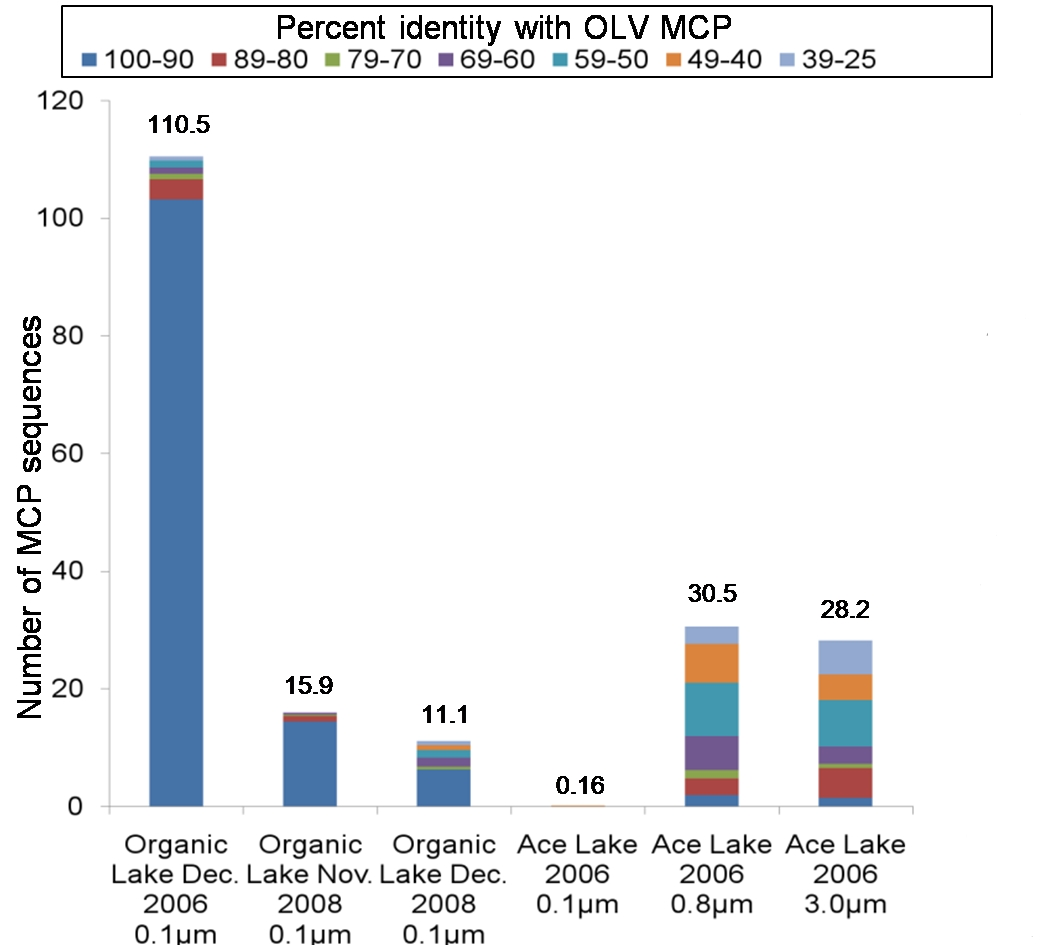
\includegraphics[width=120mm]{olv_figures/OLV_time.jpg}
\caption[Abundance and diversity of virophage capsid proteins in environmental samples]{Abundance and diversity of virophage capsid proteins in environmental samples. 
Number of \acp{ORF} from metagenomic reads that match to \ac{OLV} \ac{MCP} (\textsc{BLASTp} e-value cut-off 1e$-$5, abundance normalised to 100,000 reads per sample), and the proportion of virophage capsid types, for the Organic Lake 0.1 \textmu{}m and Ace Lake 0.1, 0.8 and 3.0 \textmu{}m fractions.  
}
\label{fig:OLV_time}

\end{figure}

\begingroup
\begin{table}
\footnotesize
\caption[\acs{OLV} \acs{MCP} in Organic Lake and Ace Lake  and \ac{CAMERA}]{ \textsc{BLASTp} matches for \ac{OLV} \ac{MCP} in predicted \acp{ORF} of Organic Lake and Ace Lake contigs and \ac{CAMERA} metagenomic read \ac{ORF} peptide database. (E-value cut-off 1e$-$5, alignment length $>$100aa). Aln., alignment length; Cov., coverage.}
\label{tab:olv_mcp_blastp}
\smallskip
\begin{tabularx}{\textwidth}{p{2.5cm}p{0.5cm}p{3.5cm}Xp{0.5cm}p{0.5cm}p{0.8cm}p{0.5cm}}
\toprule
\textbf{Sample} & \textbf{Size (\textmu{}m)} & \textbf{Gene ID} & \textbf{Scaffold ID} & \textbf{Id. (\%)} & \textbf{Aln. (aa)} & \textbf{E-value} & \textbf{Cov. ($\times$)} \\
\midrule
Organic Lake & 0.1 & OLV9 & - & - & - & - & 77.12 \\
December & 0.8 & 176157210 & scf7180000034275 & 98.61 & 575 & 0.0 & 16.03 \\
2006 & 3.0 & 181703798 & deg7180000108904 & 98.96 & 575 & 0.0 & 48.65 \\

Organic Lake & 0.1 & 192841413 & deg7180000116398 & 99.64 & 555 & 0.0 & 16.03 \\
November & 0.8 & 193037024 & scf7180000086663 & 93.98 & 133 & 2e$-$61 & 2.5 \\
2008 & 3.0 & 192638971 & deg7180000028400 & 99.36 & 156 & 1e$-$76 & 1.86 \\
 &  & 192955191 & deg7180000024244 & 93.98 & 133 & 1e$-$61 & 3.10 \\

Organic Lake & 0.1 & 192709908 & scf7180000109753 & 99.01 & 304 & 9e$-$173 & 4.38 \\
December &  & 192709920 & scf7180000109753 & 99.59 & 244 & 1e$-$120 & 4.38 \\
2008 &  & 192712009 & deg7180000067104 & 54.70 & 117 & 3e$-$30 & 1.58 \\
 &  & 192890551 & deg7180000061276 & 36.89 & 122 & 2e$-$13 & 3.15 \\
 & 0.8 & 193060302 & deg7180000053149 & 53.75 & 160 & 6e$-$43 & 2.30 \\

Ace Lake & 0.1 & 167813925 & scf7180000126822 & 28.86 & 246 & 3e$-$14 & 2.36  \\
2006 &  & 167858124 & scf7180000129064 & 21.78 & 381 & 5e$-$10 & 1.94 \\
 &  & 167891594 & scf7180000136823 & 24.85 & 326 & 2e$-$04 & 8.15 \\
 &  & 167875536 & deg7180000086604 & 22.95 & 244 & 6e$-$04 & 2.21 \\

 & 0.8 & 176091445 & deg7180000053588 & 91.61 & 143 & 8e$-$78 & 3.35 \\
 &  & 175769103 & deg7180000078701 & 88.24 & 153 & 1e$-$74 & 1.77 \\
 &  & 176042318 & deg7180000058177 & 81.77 & 181 & 1e$-$74 & 2.48 \\
 &  & 176000635 & deg7180000087166 & 53.39 & 221 & 8e$-$58 & 2.50 \\
 &  & 176042707 & deg7180000058207 & 50.78 & 193 & 5e$-$46 & 2.34 \\
 &  & 175886340 & deg7180000074162 & 58.90 & 146 & 4e$-$45 & 2.73 \\
 &  & 176249679 & deg7180000049481 & 61.94 & 155 & 2e$-$44 & 2.75 \\
 &  & 175748439 & deg7180000058552 & 76.79 & 112 & 2e$-$35 & 2.39 \\
 &  & 175637390 & deg7180000058712 & 50.91 & 165 & 2e$-$35 & 2.03 \\
 &  & 176100822 & deg7180000055966 & 53.38 & 133 & 6e$-$35 & 1.48 \\
 &  & 176018109 & deg7180000086684 & 59.68 & 124 & 4e$-$27 & 1.66 \\
 &  & 176000624 & deg7180000087165 & 53.85 & 104 & 6e$-$27 & 1.73 \\
 &  & 175805608 & deg7180000054222 & 48.60 & 107 & 7e$-$21 & 1.93 \\
 &  & 175908895 & deg7180000061971 & 51.91 & 131 & 4e$-$20 & 3.27 \\
 &  & 175821062 & deg7180000080443 & 46.46 & 127 & 6e$-$20 & 1.43 \\
 &  & 176026419 & deg7180000054364 & 52.59 & 116 & 8e$-$19 & 1.47 \\
 &  & 176133336 & scf7180000089989 & 38.36 & 146 & 3e$-$12 & 1.51 \\
 &  & 176018257 & deg7180000086719 & 31.21 & 173 & 4e$-$12 & 1.23 \\
 &  & 176137412 & deg7180000052688 & 29.37 & 126 & 1e$-$06 & 2.47 \\
 &  & 175686880 & scf7180000092161 & 24.00 & 125 & 2e$-$06 & 2.98 \\
 & 3.0 & 175741076 & deg7180000030508 & 85.78 & 232 & 8e$-$109 & 1.25 \\
 &  & 175748837 & deg7180000027929 & 55.29 & 170 & 4e$-$44 & 1.32 \\
 &  & 175751996 & deg7180000037324 & 51.27 & 158 & 5e$-$41 & 1.63 \\
 &  & 175859792 & scf7180000045944 & 30.21 & 288 & 8e$-$26 & 2.69 \\

Punta Cormorant  & 0.1 & JCVI\_PEP\_1105120114513 & - & 27.84 & 273 & 2e$-$14 & - \\
hypersaline &  & JCVI\_PEP\_1105100621559 & - & 24.76 & 307 & 9e$-$10 & - \\
lagoon (GS003) &  & JCVI\_PEP\_1105161421335 & - & 25.61 & 289 & 2e$-$6 & - \\

Delaware Bay & 0.1 & JCVI\_PEP\_1105106741177 & - & 24.62 & 264 & 6e$-$14 & - \\
(GS011)  &  & JCVI\_PEP\_1105089715877 & - & 27.16 & 313 & 1e$-$17 & - \\

Upwelling (GS031) & 0.1 & JCVI\_PEP\_1105079267881 & - & 28.23 & 170 & 8e$-$11 & - \\

Lake Gatun  & 0.1 & JCVI\_PEP\_1105119255775 & - & 26.71 & 149 & 5e$-$9 & - \\
Panama (GS020) &  &  &  &  &  &  &  \\

\bottomrule
\end{tabularx}
\end{table}
\endgroup



From surface water samples of nearby Ace Lake (meromictic, surface 2\% salinity), a large number of sequences were obtained that matched both the \ac{OLV} \ac{MCP} (\figreft{fig:OLV_time}, \figreft{fig:OLV_phylogeny} and \tabreft{tab:olv_mcp_blastp}) and \acp{PV} \cite{Lauro2011}. %Refer to chapter 1 
All Ace Lake size fractions contained matches to \ac{OLV} \ac{MCP}, some with high identity (80--100\%) and the majority with greater variation (25--80\% identity) (\figreft{fig:OLV_phylogeny} and \tabreft{tab:olv_mcp_blastp}). 
In contrast to Organic Lake where the largest number of matches was to the 0.1 \textmu{}m size fraction, the majority of Ace Lake sequences were from the larger fractions (\figreft{fig:OLV_time} and \tabreft{tab:olv_mcp_blastp}). 
This indicates the Ace Lake virophages were associated with host cells during sampling, or possibly with helper viruses that are larger than the \acp{OLPV}. 
\begin{figure}
\centering
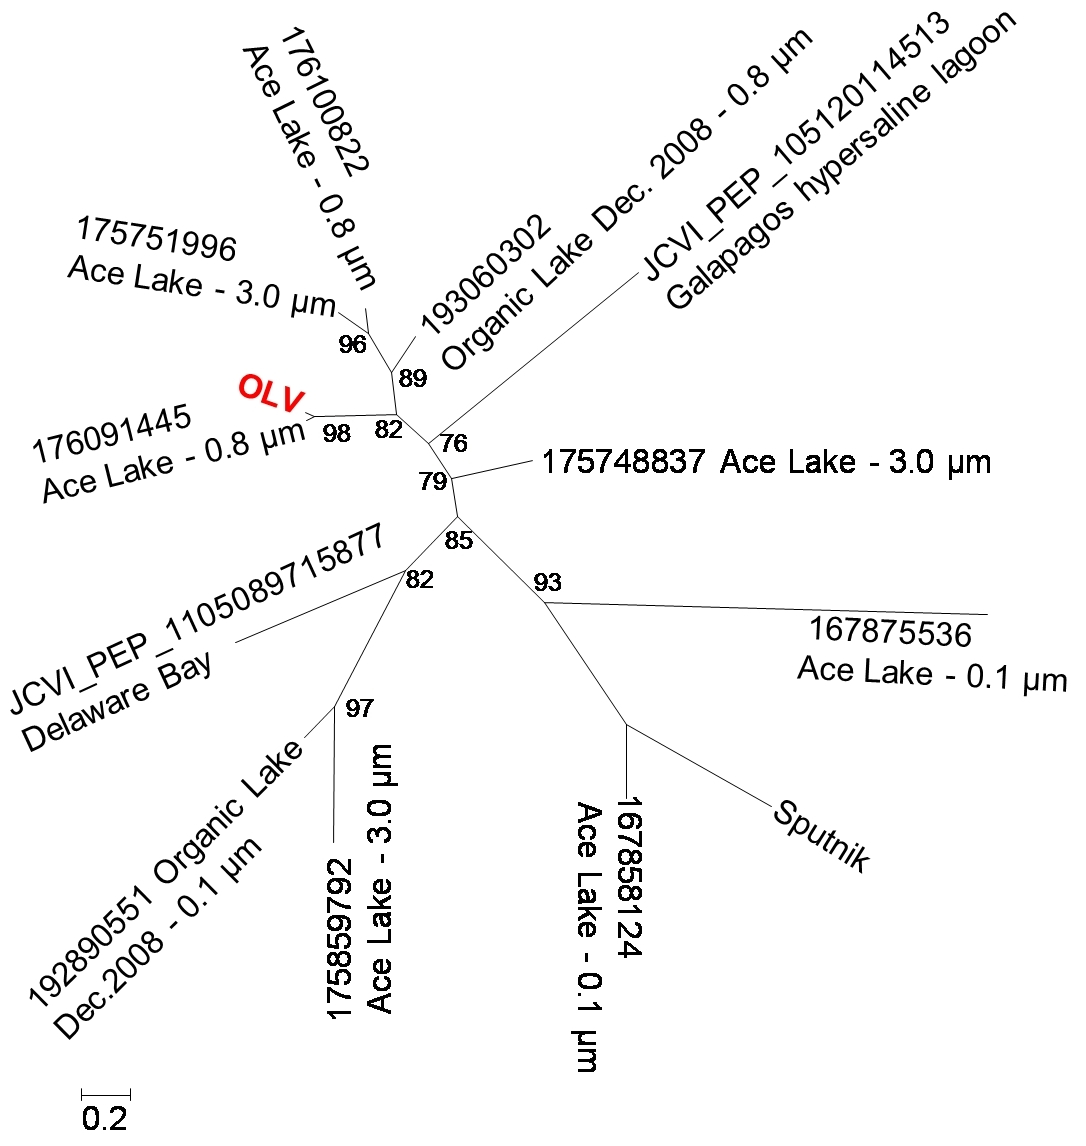
\includegraphics[width=100mm]{olv_figures/OLV_phylogeny.jpg}
\caption[Phylogeny of virophage capsid proteins]{Maximum likelihood phylogenetic tree of a conserved 103 aa region of the \ac{MCP} from Organic Lake, Ace Lake and \ac{GOS} metagenome data and Sputnik. 
}
\label{fig:OLV_phylogeny}

\end{figure}


Extending the \ac{OLV} \ac{MCP} search to the \ac{GOS} data revealed matches (25--28\% identity) to sequences from the hypersaline Punta Cormorant Lagoon (Floreana Island, Galapagos), an oceanic upwelling near Fernandina Island (Galapagos), Delaware Bay estuary (\textsc{NJ}, \textsc{USA}), and freshwater Lake Gatun (Panama) (\tabreft{tab:olv_mcp_blastp}). 
The phylogenetic analysis of a conserved 103 amino acid region of the \acp{MCP} revealed a number of clusters, with Sputnik clustering with virophage sequences from Ace Lake that had low identity (22\%) to \ac{OLV} \ac{MCP} \figref{fig:OLV_phylogeny}. 
To improve searches for virophages and better understand their physiology and evolution, it will be valuable to target more genomes (e.g. the Ace Lake 167858124 relative with 40\% MCP identity to Sputnik) and determine which genes are core to virophages and what relationship exists between genome complement and \ac{MCP} identity.
 
In view of the implications of the virophage modelling \figref{fig:LV}, the abundance and persistence of \ac{OLV} in Organic Lake and the presence of diverse virophage signatures in a variety of lake systems (fresh to hypersaline), an estuary, an ocean upwelling site and a water cooling tower (Sputnik), our study indicates that numerous types of virophages exist and play a previously unrecognised role in regulating host--virus interactions and influencing ecosystem function in aquatic environments. 

%------------------------------------------------------------------------------------------------------

\section{Acknowledgements}
We thank Craig Venter, John Bowman, Louise (Cromer) Newman, Anthony Hull, John Rich and Martin Riddle for providing helpful discussion and logistical support associated with the Antarctic expedition, and Lisa Ziegler for discussion about marine viruses. 
We acknowledge technical support for computing infrastructure and software development from Intersect, and in particular assistance from Joachim Mai. 
This work was supported by the Australian Research Council and the Australian Antarctic Division. 
Funding for sequencing was provided by the Gordon and Betty Moore Foundation to the J. Craig Venter Institute. 
Mass spectrometric results were obtained at the Bioanalytical Mass Spectrometry Facility within the Analytical Centre of the University of New South Wales. 
This work was undertaken using infrastructure provided by NSW Government co-investment in the National Collaborative Research Infrastructure Scheme. 
Subsidized access to this facility is gratefully acknowledged. 
We thank Jenny Norman from the UNSW Electron Microscopy Unit her assistance in generating images. 
